\documentclass[twoside]{book}

% Packages required by doxygen
\usepackage{fixltx2e}
\usepackage{calc}
\usepackage{doxygen}
\usepackage[export]{adjustbox} % also loads graphicx
\usepackage{graphicx}
\usepackage[utf8]{inputenc}
\usepackage{makeidx}
\usepackage{multicol}
\usepackage{multirow}
\PassOptionsToPackage{warn}{textcomp}
\usepackage{textcomp}
\usepackage[nointegrals]{wasysym}
\usepackage[table]{xcolor}

% Font selection
\usepackage[T1]{fontenc}
\usepackage[scaled=.90]{helvet}
\usepackage{courier}
\usepackage{amssymb}
\usepackage{sectsty}
\renewcommand{\familydefault}{\sfdefault}
\allsectionsfont{%
  \fontseries{bc}\selectfont%
  \color{darkgray}%
}
\renewcommand{\DoxyLabelFont}{%
  \fontseries{bc}\selectfont%
  \color{darkgray}%
}
\newcommand{\+}{\discretionary{\mbox{\scriptsize$\hookleftarrow$}}{}{}}

% Page & text layout
\usepackage{geometry}
\geometry{%
  a4paper,%
  top=2.5cm,%
  bottom=2.5cm,%
  left=2.5cm,%
  right=2.5cm%
}
\tolerance=750
\hfuzz=15pt
\hbadness=750
\setlength{\emergencystretch}{15pt}
\setlength{\parindent}{0cm}
\setlength{\parskip}{3ex plus 2ex minus 2ex}
\makeatletter
\renewcommand{\paragraph}{%
  \@startsection{paragraph}{4}{0ex}{-1.0ex}{1.0ex}{%
    \normalfont\normalsize\bfseries\SS@parafont%
  }%
}
\renewcommand{\subparagraph}{%
  \@startsection{subparagraph}{5}{0ex}{-1.0ex}{1.0ex}{%
    \normalfont\normalsize\bfseries\SS@subparafont%
  }%
}
\makeatother

% Headers & footers
\usepackage{fancyhdr}
\pagestyle{fancyplain}
\fancyhead[LE]{\fancyplain{}{\bfseries\thepage}}
\fancyhead[CE]{\fancyplain{}{}}
\fancyhead[RE]{\fancyplain{}{\bfseries\leftmark}}
\fancyhead[LO]{\fancyplain{}{\bfseries\rightmark}}
\fancyhead[CO]{\fancyplain{}{}}
\fancyhead[RO]{\fancyplain{}{\bfseries\thepage}}
\fancyfoot[LE]{\fancyplain{}{}}
\fancyfoot[CE]{\fancyplain{}{}}
\fancyfoot[RE]{\fancyplain{}{\bfseries\scriptsize Generated by Doxygen }}
\fancyfoot[LO]{\fancyplain{}{\bfseries\scriptsize Generated by Doxygen }}
\fancyfoot[CO]{\fancyplain{}{}}
\fancyfoot[RO]{\fancyplain{}{}}
\renewcommand{\footrulewidth}{0.4pt}
\renewcommand{\chaptermark}[1]{%
  \markboth{#1}{}%
}
\renewcommand{\sectionmark}[1]{%
  \markright{\thesection\ #1}%
}

% Indices & bibliography
\usepackage{natbib}
\usepackage[titles]{tocloft}
\setcounter{tocdepth}{3}
\setcounter{secnumdepth}{5}
\makeindex

% Hyperlinks (required, but should be loaded last)
\usepackage{ifpdf}
\ifpdf
  \usepackage[pdftex,pagebackref=true]{hyperref}
\else
  \usepackage[ps2pdf,pagebackref=true]{hyperref}
\fi
\hypersetup{%
  colorlinks=true,%
  linkcolor=blue,%
  citecolor=blue,%
  unicode%
}

% Custom commands
\newcommand{\clearemptydoublepage}{%
  \newpage{\pagestyle{empty}\cleardoublepage}%
}

\usepackage{caption}
\captionsetup{labelsep=space,justification=centering,font={bf},singlelinecheck=off,skip=4pt,position=top}

%===== C O N T E N T S =====

\begin{document}

% Titlepage & ToC
\hypersetup{pageanchor=false,
             bookmarksnumbered=true,
             pdfencoding=unicode
            }
\pagenumbering{alph}
\begin{titlepage}
\vspace*{7cm}
\begin{center}%
{\Large My Project }\\
\vspace*{1cm}
{\large Generated by Doxygen 1.8.14}\\
\end{center}
\end{titlepage}
\clearemptydoublepage
\pagenumbering{roman}
\tableofcontents
\clearemptydoublepage
\pagenumbering{arabic}
\hypersetup{pageanchor=true}

%--- Begin generated contents ---
\chapter{Class Index}
\section{Class List}
Here are the classes, structs, unions and interfaces with brief descriptions\+:\begin{DoxyCompactList}
\item\contentsline{section}{\mbox{\hyperlink{class_face}{Face}} \\*Holds objects that are used to describe the faces in rendering the 3d model using open\+GL }{\pageref{class_face}}{}
\item\contentsline{section}{\mbox{\hyperlink{class_glwidget}{Glwidget}} }{\pageref{class_glwidget}}{}
\item\contentsline{section}{\mbox{\hyperlink{class_main_window}{Main\+Window}} }{\pageref{class_main_window}}{}
\item\contentsline{section}{\mbox{\hyperlink{class_model}{Model}} }{\pageref{class_model}}{}
\item\contentsline{section}{\mbox{\hyperlink{class_model2d}{Model2d}} \\*Creates the 2d model for a particular design by defining the necessary attributes }{\pageref{class_model2d}}{}
\item\contentsline{section}{\mbox{\hyperlink{class_projection}{Projection}} }{\pageref{class_projection}}{}
\item\contentsline{section}{\mbox{\hyperlink{class_projection_x}{ProjectionX}} \\*Defines the projectionX for the current design to be displayed using the model class }{\pageref{class_projection_x}}{}
\item\contentsline{section}{\mbox{\hyperlink{class_projection_y}{ProjectionY}} \\*Defines the projectionY for the current design to be displayed using the model class }{\pageref{class_projection_y}}{}
\item\contentsline{section}{\mbox{\hyperlink{class_projection_z}{ProjectionZ}} \\*Defines the projectionZ for the current design to be displayed using the model class }{\pageref{class_projection_z}}{}
\item\contentsline{section}{\mbox{\hyperlink{class_sample_models}{Sample\+Models}} \\*Defines the templates for the software including other necessary designs for base display like the axes }{\pageref{class_sample_models}}{}
\end{DoxyCompactList}

\chapter{File Index}
\section{File List}
Here is a list of all files with brief descriptions\+:\begin{DoxyCompactList}
\item\contentsline{section}{src/\mbox{\hyperlink{glwidget_8cpp}{glwidget.\+cpp}} }{\pageref{glwidget_8cpp}}{}
\item\contentsline{section}{src/\mbox{\hyperlink{glwidget_8h}{glwidget.\+h}} }{\pageref{glwidget_8h}}{}
\item\contentsline{section}{src/\mbox{\hyperlink{main_8cpp}{main.\+cpp}} }{\pageref{main_8cpp}}{}
\item\contentsline{section}{src/\mbox{\hyperlink{mainwindow_8cpp}{mainwindow.\+cpp}} }{\pageref{mainwindow_8cpp}}{}
\item\contentsline{section}{src/\mbox{\hyperlink{mainwindow_8h}{mainwindow.\+h}} }{\pageref{mainwindow_8h}}{}
\item\contentsline{section}{src/\mbox{\hyperlink{model_8cpp}{model.\+cpp}} }{\pageref{model_8cpp}}{}
\item\contentsline{section}{src/\mbox{\hyperlink{model_8h}{model.\+h}} }{\pageref{model_8h}}{}
\item\contentsline{section}{src/\mbox{\hyperlink{model2d_8cpp}{model2d.\+cpp}} }{\pageref{model2d_8cpp}}{}
\item\contentsline{section}{src/\mbox{\hyperlink{model2d_8h}{model2d.\+h}} }{\pageref{model2d_8h}}{}
\item\contentsline{section}{src/\mbox{\hyperlink{projectionx_8cpp}{projectionx.\+cpp}} }{\pageref{projectionx_8cpp}}{}
\item\contentsline{section}{src/\mbox{\hyperlink{projectionx_8h}{projectionx.\+h}} }{\pageref{projectionx_8h}}{}
\item\contentsline{section}{src/\mbox{\hyperlink{projectiony_8cpp}{projectiony.\+cpp}} }{\pageref{projectiony_8cpp}}{}
\item\contentsline{section}{src/\mbox{\hyperlink{projectiony_8h}{projectiony.\+h}} }{\pageref{projectiony_8h}}{}
\item\contentsline{section}{src/\mbox{\hyperlink{projectionz_8cpp}{projectionz.\+cpp}} }{\pageref{projectionz_8cpp}}{}
\item\contentsline{section}{src/\mbox{\hyperlink{projectionz_8h}{projectionz.\+h}} }{\pageref{projectionz_8h}}{}
\item\contentsline{section}{src/\mbox{\hyperlink{samplemodels_8cpp}{samplemodels.\+cpp}} }{\pageref{samplemodels_8cpp}}{}
\item\contentsline{section}{src/\mbox{\hyperlink{samplemodels_8h}{samplemodels.\+h}} }{\pageref{samplemodels_8h}}{}
\item\contentsline{section}{src/\mbox{\hyperlink{window2d_8cpp}{window2d.\+cpp}} }{\pageref{window2d_8cpp}}{}
\end{DoxyCompactList}

\chapter{Class Documentation}
\hypertarget{class_direction_cosines}{}\section{Direction\+Cosines Class Reference}
\label{class_direction_cosines}\index{Direction\+Cosines@{Direction\+Cosines}}


Class to define the direction cosines in 3d space.  




{\ttfamily \#include $<$Direction\+Cosines.\+hpp$>$}

\subsection*{Public Member Functions}
\begin{DoxyCompactItemize}
\item 
\mbox{\hyperlink{class_direction_cosines_a0b0eae6aaa802ed4eed8a163a7da960a}{Direction\+Cosine}} (float a, float b, float c)
\begin{DoxyCompactList}\small\item\em Class might be initialized with direction cosines or ratios, to make it inclusive of both. \end{DoxyCompactList}\item 
\mbox{\hyperlink{class_direction_cosines_a595e87c5e381f0d877eee26ba75283c7}{$\sim$\+Direction\+Cosines}} ()
\item 
float \mbox{\hyperlink{class_direction_cosines_a734a1153319e8e5b16d794085a74fe21}{dot\+Product}} (\mbox{\hyperlink{class_direction_cosines_a0b0eae6aaa802ed4eed8a163a7da960a}{Direction\+Cosine}} l)
\item 
\mbox{\hyperlink{class_direction_cosines_a0b0eae6aaa802ed4eed8a163a7da960a}{Direction\+Cosine}} \mbox{\hyperlink{class_direction_cosines_afc5844a79ed93bc86c96ce5c303d816a}{cross\+Product}} (\mbox{\hyperlink{class_direction_cosines_a0b0eae6aaa802ed4eed8a163a7da960a}{Direction\+Cosine}} l)
\end{DoxyCompactItemize}
\subsection*{Public Attributes}
\begin{DoxyCompactItemize}
\item 
float \mbox{\hyperlink{class_direction_cosines_a6fde43a3e699635fecf3296c72fe7045}{xl}}
\begin{DoxyCompactList}\small\item\em cosine of the angle made by the line/segment with the x-\/axis \end{DoxyCompactList}\item 
float \mbox{\hyperlink{class_direction_cosines_a277b009af5e287e276d445a6aecef108}{yl}}
\begin{DoxyCompactList}\small\item\em cosine of the angle made by the line/segment with the y-\/axis \end{DoxyCompactList}\item 
float \mbox{\hyperlink{class_direction_cosines_afb263bbd031ba13d68380e367403ec65}{zl}}
\begin{DoxyCompactList}\small\item\em cosine of the angle made by the line/segment with the z-\/axis \end{DoxyCompactList}\end{DoxyCompactItemize}


\subsection{Detailed Description}
Class to define the direction cosines in 3d space. 

\subsection{Constructor \& Destructor Documentation}
\mbox{\Hypertarget{class_direction_cosines_a595e87c5e381f0d877eee26ba75283c7}\label{class_direction_cosines_a595e87c5e381f0d877eee26ba75283c7}} 
\index{Direction\+Cosines@{Direction\+Cosines}!````~Direction\+Cosines@{$\sim$\+Direction\+Cosines}}
\index{````~Direction\+Cosines@{$\sim$\+Direction\+Cosines}!Direction\+Cosines@{Direction\+Cosines}}
\subsubsection{\texorpdfstring{$\sim$\+Direction\+Cosines()}{~DirectionCosines()}}
{\footnotesize\ttfamily Direction\+Cosines\+::$\sim$\+Direction\+Cosines (\begin{DoxyParamCaption}{ }\end{DoxyParamCaption})}



\subsection{Member Function Documentation}
\mbox{\Hypertarget{class_direction_cosines_afc5844a79ed93bc86c96ce5c303d816a}\label{class_direction_cosines_afc5844a79ed93bc86c96ce5c303d816a}} 
\index{Direction\+Cosines@{Direction\+Cosines}!cross\+Product@{cross\+Product}}
\index{cross\+Product@{cross\+Product}!Direction\+Cosines@{Direction\+Cosines}}
\subsubsection{\texorpdfstring{cross\+Product()}{crossProduct()}}
{\footnotesize\ttfamily \mbox{\hyperlink{class_direction_cosines}{Direction\+Cosines}} Direction\+Cosines\+::cross\+Product (\begin{DoxyParamCaption}\item[{\mbox{\hyperlink{class_direction_cosines_a0b0eae6aaa802ed4eed8a163a7da960a}{Direction\+Cosine}}}]{l }\end{DoxyParamCaption})}

\mbox{\Hypertarget{class_direction_cosines_a0b0eae6aaa802ed4eed8a163a7da960a}\label{class_direction_cosines_a0b0eae6aaa802ed4eed8a163a7da960a}} 
\index{Direction\+Cosines@{Direction\+Cosines}!Direction\+Cosine@{Direction\+Cosine}}
\index{Direction\+Cosine@{Direction\+Cosine}!Direction\+Cosines@{Direction\+Cosines}}
\subsubsection{\texorpdfstring{Direction\+Cosine()}{DirectionCosine()}}
{\footnotesize\ttfamily Direction\+Cosines\+::\+Direction\+Cosine (\begin{DoxyParamCaption}\item[{float}]{a,  }\item[{float}]{b,  }\item[{float}]{c }\end{DoxyParamCaption})}



Class might be initialized with direction cosines or ratios, to make it inclusive of both. 

\mbox{\Hypertarget{class_direction_cosines_a734a1153319e8e5b16d794085a74fe21}\label{class_direction_cosines_a734a1153319e8e5b16d794085a74fe21}} 
\index{Direction\+Cosines@{Direction\+Cosines}!dot\+Product@{dot\+Product}}
\index{dot\+Product@{dot\+Product}!Direction\+Cosines@{Direction\+Cosines}}
\subsubsection{\texorpdfstring{dot\+Product()}{dotProduct()}}
{\footnotesize\ttfamily float Direction\+Cosines\+::dot\+Product (\begin{DoxyParamCaption}\item[{\mbox{\hyperlink{class_direction_cosines_a0b0eae6aaa802ed4eed8a163a7da960a}{Direction\+Cosine}}}]{l }\end{DoxyParamCaption})}



\subsection{Member Data Documentation}
\mbox{\Hypertarget{class_direction_cosines_a6fde43a3e699635fecf3296c72fe7045}\label{class_direction_cosines_a6fde43a3e699635fecf3296c72fe7045}} 
\index{Direction\+Cosines@{Direction\+Cosines}!xl@{xl}}
\index{xl@{xl}!Direction\+Cosines@{Direction\+Cosines}}
\subsubsection{\texorpdfstring{xl}{xl}}
{\footnotesize\ttfamily float Direction\+Cosines\+::xl}



cosine of the angle made by the line/segment with the x-\/axis 

\mbox{\Hypertarget{class_direction_cosines_a277b009af5e287e276d445a6aecef108}\label{class_direction_cosines_a277b009af5e287e276d445a6aecef108}} 
\index{Direction\+Cosines@{Direction\+Cosines}!yl@{yl}}
\index{yl@{yl}!Direction\+Cosines@{Direction\+Cosines}}
\subsubsection{\texorpdfstring{yl}{yl}}
{\footnotesize\ttfamily float Direction\+Cosines\+::yl}



cosine of the angle made by the line/segment with the y-\/axis 

\mbox{\Hypertarget{class_direction_cosines_afb263bbd031ba13d68380e367403ec65}\label{class_direction_cosines_afb263bbd031ba13d68380e367403ec65}} 
\index{Direction\+Cosines@{Direction\+Cosines}!zl@{zl}}
\index{zl@{zl}!Direction\+Cosines@{Direction\+Cosines}}
\subsubsection{\texorpdfstring{zl}{zl}}
{\footnotesize\ttfamily float Direction\+Cosines\+::zl}



cosine of the angle made by the line/segment with the z-\/axis 



The documentation for this class was generated from the following files\+:\begin{DoxyCompactItemize}
\item 
\mbox{\hyperlink{_direction_cosines_8hpp}{Direction\+Cosines.\+hpp}}\item 
\mbox{\hyperlink{_direction_cosines_8cpp}{Direction\+Cosines.\+cpp}}\end{DoxyCompactItemize}

\hypertarget{class_graph}{}\section{Graph Class Reference}
\label{class_graph}\index{Graph@{Graph}}


A \mbox{\hyperlink{class_graph}{Graph}} Class to model a 3D or a 2D view. Determine whether to use an Adjcancey List or Adjanceny Matrix representation.  




{\ttfamily \#include $<$Graph.\+hpp$>$}

\subsection*{Public Member Functions}
\begin{DoxyCompactItemize}
\item 
\mbox{\hyperlink{class_graph_ae4c72b8ac4d693c49800a4c7e273654f}{Graph}} ()
\begin{DoxyCompactList}\small\item\em Constructor for \mbox{\hyperlink{class_graph}{Graph}} object. \end{DoxyCompactList}\item 
\mbox{\hyperlink{class_graph_a902c5b3eacb66d60752525ab23297a95}{$\sim$\+Graph}} ()
\begin{DoxyCompactList}\small\item\em Destructor for \mbox{\hyperlink{class_graph}{Graph}} object. \end{DoxyCompactList}\item 
bool \mbox{\hyperlink{class_graph_ae807fc072ac3e93c9718ee326a0d0822}{contains\+Node}} (\mbox{\hyperlink{class_point}{Point}} P)
\begin{DoxyCompactList}\small\item\em Returns True if it contains the specified Node else False. \end{DoxyCompactList}\item 
bool \mbox{\hyperlink{class_graph_af7eefeaacac324886fa73f3a2e85f20a}{contains\+Edge}} (\mbox{\hyperlink{class_line}{Line}} E)
\begin{DoxyCompactList}\small\item\em Returns True if it contains the specified Node else False. \end{DoxyCompactList}\item 
void \mbox{\hyperlink{class_graph_aaf5ccb68d053bd64b6b057783c99608c}{add\+Node}} (\mbox{\hyperlink{class_point}{Point}} P)
\begin{DoxyCompactList}\small\item\em adds a node to the \mbox{\hyperlink{class_graph}{Graph}} \end{DoxyCompactList}\item 
void \mbox{\hyperlink{class_graph_a5c30bae1d7a0bbb2f9d9f0d5ad40f78f}{add\+Edge}} (\mbox{\hyperlink{class_line}{Line}} E)
\begin{DoxyCompactList}\small\item\em adds an edge to the \mbox{\hyperlink{class_graph}{Graph}} \end{DoxyCompactList}\item 
void \mbox{\hyperlink{class_graph_a285f720a5e75fc099dcc32fd4a37786a}{update\+Node}} (\mbox{\hyperlink{class_point}{Point}} P1, \mbox{\hyperlink{class_point}{Point}} P2)
\begin{DoxyCompactList}\small\item\em updates a Node in the \mbox{\hyperlink{class_graph}{Graph}} \end{DoxyCompactList}\item 
void \mbox{\hyperlink{class_graph_a74d50f92f6f2291675020e038132c85f}{delete\+Node}} (\mbox{\hyperlink{class_point}{Point}} P)
\begin{DoxyCompactList}\small\item\em deletes a node from the \mbox{\hyperlink{class_graph}{Graph}} \end{DoxyCompactList}\item 
void \mbox{\hyperlink{class_graph_a39031d4b9f6527501333e612cb91cca6}{delete\+Edge}} (Edge E)
\begin{DoxyCompactList}\small\item\em deletes an edge from the \mbox{\hyperlink{class_graph}{Graph}} \end{DoxyCompactList}\end{DoxyCompactItemize}
\subsection*{Public Attributes}
\begin{DoxyCompactItemize}
\item 
list$<$ \mbox{\hyperlink{class_point}{Point}} $>$ \mbox{\hyperlink{class_graph_abbffb935f6c2c6723a149d70bdb0762f}{Node}}
\begin{DoxyCompactList}\small\item\em the abstract Node data member that describes the corners/vertices of the View \end{DoxyCompactList}\item 
list$<$ \mbox{\hyperlink{class_line}{Line}} $>$ \mbox{\hyperlink{class_graph_aa8bbd434abc0c7a804ad7687b3ec2511}{Edge\+Set}}
\begin{DoxyCompactList}\small\item\em the abstract Edge\+Set data member that describes the solid/dashed edges of the View \end{DoxyCompactList}\end{DoxyCompactItemize}


\subsection{Detailed Description}
A \mbox{\hyperlink{class_graph}{Graph}} Class to model a 3D or a 2D view. Determine whether to use an Adjcancey List or Adjanceny Matrix representation. 

\subsection{Constructor \& Destructor Documentation}
\mbox{\Hypertarget{class_graph_ae4c72b8ac4d693c49800a4c7e273654f}\label{class_graph_ae4c72b8ac4d693c49800a4c7e273654f}} 
\index{Graph@{Graph}!Graph@{Graph}}
\index{Graph@{Graph}!Graph@{Graph}}
\subsubsection{\texorpdfstring{Graph()}{Graph()}}
{\footnotesize\ttfamily Graph\+::\+Graph (\begin{DoxyParamCaption}{ }\end{DoxyParamCaption})}



Constructor for \mbox{\hyperlink{class_graph}{Graph}} object. 

\mbox{\Hypertarget{class_graph_a902c5b3eacb66d60752525ab23297a95}\label{class_graph_a902c5b3eacb66d60752525ab23297a95}} 
\index{Graph@{Graph}!````~Graph@{$\sim$\+Graph}}
\index{````~Graph@{$\sim$\+Graph}!Graph@{Graph}}
\subsubsection{\texorpdfstring{$\sim$\+Graph()}{~Graph()}}
{\footnotesize\ttfamily Graph\+::$\sim$\+Graph (\begin{DoxyParamCaption}{ }\end{DoxyParamCaption})}



Destructor for \mbox{\hyperlink{class_graph}{Graph}} object. 



\subsection{Member Function Documentation}
\mbox{\Hypertarget{class_graph_a5c30bae1d7a0bbb2f9d9f0d5ad40f78f}\label{class_graph_a5c30bae1d7a0bbb2f9d9f0d5ad40f78f}} 
\index{Graph@{Graph}!add\+Edge@{add\+Edge}}
\index{add\+Edge@{add\+Edge}!Graph@{Graph}}
\subsubsection{\texorpdfstring{add\+Edge()}{addEdge()}}
{\footnotesize\ttfamily void Graph\+::add\+Edge (\begin{DoxyParamCaption}\item[{\mbox{\hyperlink{class_line}{Line}}}]{E }\end{DoxyParamCaption})}



adds an edge to the \mbox{\hyperlink{class_graph}{Graph}} 

\mbox{\Hypertarget{class_graph_aaf5ccb68d053bd64b6b057783c99608c}\label{class_graph_aaf5ccb68d053bd64b6b057783c99608c}} 
\index{Graph@{Graph}!add\+Node@{add\+Node}}
\index{add\+Node@{add\+Node}!Graph@{Graph}}
\subsubsection{\texorpdfstring{add\+Node()}{addNode()}}
{\footnotesize\ttfamily void Graph\+::add\+Node (\begin{DoxyParamCaption}\item[{\mbox{\hyperlink{class_point}{Point}}}]{P }\end{DoxyParamCaption})}



adds a node to the \mbox{\hyperlink{class_graph}{Graph}} 

\mbox{\Hypertarget{class_graph_af7eefeaacac324886fa73f3a2e85f20a}\label{class_graph_af7eefeaacac324886fa73f3a2e85f20a}} 
\index{Graph@{Graph}!contains\+Edge@{contains\+Edge}}
\index{contains\+Edge@{contains\+Edge}!Graph@{Graph}}
\subsubsection{\texorpdfstring{contains\+Edge()}{containsEdge()}}
{\footnotesize\ttfamily bool Graph\+::contains\+Edge (\begin{DoxyParamCaption}\item[{\mbox{\hyperlink{class_line}{Line}}}]{E }\end{DoxyParamCaption})}



Returns True if it contains the specified Node else False. 

\mbox{\Hypertarget{class_graph_ae807fc072ac3e93c9718ee326a0d0822}\label{class_graph_ae807fc072ac3e93c9718ee326a0d0822}} 
\index{Graph@{Graph}!contains\+Node@{contains\+Node}}
\index{contains\+Node@{contains\+Node}!Graph@{Graph}}
\subsubsection{\texorpdfstring{contains\+Node()}{containsNode()}}
{\footnotesize\ttfamily bool Graph\+::contains\+Node (\begin{DoxyParamCaption}\item[{\mbox{\hyperlink{class_point}{Point}}}]{P }\end{DoxyParamCaption})}



Returns True if it contains the specified Node else False. 

\mbox{\Hypertarget{class_graph_a39031d4b9f6527501333e612cb91cca6}\label{class_graph_a39031d4b9f6527501333e612cb91cca6}} 
\index{Graph@{Graph}!delete\+Edge@{delete\+Edge}}
\index{delete\+Edge@{delete\+Edge}!Graph@{Graph}}
\subsubsection{\texorpdfstring{delete\+Edge()}{deleteEdge()}}
{\footnotesize\ttfamily void Graph\+::delete\+Edge (\begin{DoxyParamCaption}\item[{Edge}]{E }\end{DoxyParamCaption})}



deletes an edge from the \mbox{\hyperlink{class_graph}{Graph}} 

\mbox{\Hypertarget{class_graph_a74d50f92f6f2291675020e038132c85f}\label{class_graph_a74d50f92f6f2291675020e038132c85f}} 
\index{Graph@{Graph}!delete\+Node@{delete\+Node}}
\index{delete\+Node@{delete\+Node}!Graph@{Graph}}
\subsubsection{\texorpdfstring{delete\+Node()}{deleteNode()}}
{\footnotesize\ttfamily void Graph\+::delete\+Node (\begin{DoxyParamCaption}\item[{\mbox{\hyperlink{class_point}{Point}}}]{P }\end{DoxyParamCaption})}



deletes a node from the \mbox{\hyperlink{class_graph}{Graph}} 

\mbox{\Hypertarget{class_graph_a285f720a5e75fc099dcc32fd4a37786a}\label{class_graph_a285f720a5e75fc099dcc32fd4a37786a}} 
\index{Graph@{Graph}!update\+Node@{update\+Node}}
\index{update\+Node@{update\+Node}!Graph@{Graph}}
\subsubsection{\texorpdfstring{update\+Node()}{updateNode()}}
{\footnotesize\ttfamily void Graph\+::update\+Node (\begin{DoxyParamCaption}\item[{\mbox{\hyperlink{class_point}{Point}}}]{P1,  }\item[{\mbox{\hyperlink{class_point}{Point}}}]{P2 }\end{DoxyParamCaption})}



updates a Node in the \mbox{\hyperlink{class_graph}{Graph}} 



\subsection{Member Data Documentation}
\mbox{\Hypertarget{class_graph_aa8bbd434abc0c7a804ad7687b3ec2511}\label{class_graph_aa8bbd434abc0c7a804ad7687b3ec2511}} 
\index{Graph@{Graph}!Edge\+Set@{Edge\+Set}}
\index{Edge\+Set@{Edge\+Set}!Graph@{Graph}}
\subsubsection{\texorpdfstring{Edge\+Set}{EdgeSet}}
{\footnotesize\ttfamily list$<$\mbox{\hyperlink{class_line}{Line}}$>$ Graph\+::\+Edge\+Set}



the abstract Edge\+Set data member that describes the solid/dashed edges of the View 

\mbox{\Hypertarget{class_graph_abbffb935f6c2c6723a149d70bdb0762f}\label{class_graph_abbffb935f6c2c6723a149d70bdb0762f}} 
\index{Graph@{Graph}!Node@{Node}}
\index{Node@{Node}!Graph@{Graph}}
\subsubsection{\texorpdfstring{Node}{Node}}
{\footnotesize\ttfamily list$<$\mbox{\hyperlink{class_point}{Point}}$>$ Graph\+::\+Node}



the abstract Node data member that describes the corners/vertices of the View 



The documentation for this class was generated from the following files\+:\begin{DoxyCompactItemize}
\item 
\mbox{\hyperlink{_graph_8hpp}{Graph.\+hpp}}\item 
\mbox{\hyperlink{_graph_8cpp}{Graph.\+cpp}}\end{DoxyCompactItemize}

\hypertarget{class_line}{}\section{Line Class Reference}
\label{class_line}\index{Line@{Line}}


A Class to define a line in the space 2\+D/3D.  




{\ttfamily \#include $<$Line.\+hpp$>$}

\subsection*{Public Member Functions}
\begin{DoxyCompactItemize}
\item 
\mbox{\hyperlink{class_line_ae24f583f6e61000f88a20205e9b7cf1c}{Line}} (\mbox{\hyperlink{class_direction_cosines}{Direction\+Cosines}} dc, \mbox{\hyperlink{class_point}{Point}} \mbox{\hyperlink{class_line_ade526d53a83ae2cfad4472affeb9ce8d}{p}})
\begin{DoxyCompactList}\small\item\em Constructor for line of the form of direction cosines and a point. \end{DoxyCompactList}\item 
\mbox{\hyperlink{class_line_afeaa676c7d249d582c5766dc732a78e2}{Line}} (\mbox{\hyperlink{class_point}{Point}} p1, \mbox{\hyperlink{class_point}{Point}} p2)
\begin{DoxyCompactList}\small\item\em Constructor for line of the form of two points p1, p2. \end{DoxyCompactList}\item 
\mbox{\hyperlink{class_line_aabe85f48d22d92b62257091f48174fac}{$\sim$\+Line}} ()
\begin{DoxyCompactList}\small\item\em Destructor for line object. \end{DoxyCompactList}\item 
bool \mbox{\hyperlink{class_line_a8059ce73fc21fafe0ea87939d7d20895}{is\+Parallel}} (\mbox{\hyperlink{class_line}{Line}} L)
\begin{DoxyCompactList}\small\item\em Returns True when line is parallel to given line. \end{DoxyCompactList}\item 
bool \mbox{\hyperlink{class_line_adf08ea54b857c27d783321a3e6858222}{is\+Perpendicular}} (\mbox{\hyperlink{class_line}{Line}} L)
\begin{DoxyCompactList}\small\item\em Returns True when line is perpendicular to given line. \end{DoxyCompactList}\item 
float \mbox{\hyperlink{class_line_aefe5ec3e42ab38c1f60e65ca09f0fd29}{angle\+With\+Line}} (\mbox{\hyperlink{class_line}{Line}} L)
\begin{DoxyCompactList}\small\item\em Returns angle made with given \mbox{\hyperlink{class_line}{Line}}. \end{DoxyCompactList}\item 
float \mbox{\hyperlink{class_line_abd11dc16386ee1d5424deac55dea0d1b}{angle\+With\+Plane}} (\mbox{\hyperlink{class_plane}{Plane}} P)
\begin{DoxyCompactList}\small\item\em Returns angle made with given \mbox{\hyperlink{class_plane}{Plane}}. \end{DoxyCompactList}\item 
\mbox{\hyperlink{class_line}{Line}} \mbox{\hyperlink{class_line_af20457df1ce948794350fab12c16ee14}{projection\+On\+Plane}} (\mbox{\hyperlink{class_plane}{Plane}} P)
\begin{DoxyCompactList}\small\item\em Returns projection of line on the given \mbox{\hyperlink{class_plane}{Plane}}. \end{DoxyCompactList}\item 
\mbox{\hyperlink{class_line}{Line}} \mbox{\hyperlink{class_line_a12787f5d97b7764c5b1836fb9007fb86}{image\+In\+Plane}} (\mbox{\hyperlink{class_plane}{Plane}} P)
\begin{DoxyCompactList}\small\item\em Returns image of line in the given \mbox{\hyperlink{class_plane}{Plane}}. \end{DoxyCompactList}\item 
bool \mbox{\hyperlink{class_line_aad7d2a0b6ac395a1bd81d55dd2b7a81d}{lies\+In\+Plane}} (\mbox{\hyperlink{class_plane}{Plane}} P)
\begin{DoxyCompactList}\small\item\em Returns True if line lies in the given \mbox{\hyperlink{class_plane}{Plane}}. \end{DoxyCompactList}\item 
bool \mbox{\hyperlink{class_line_a01b3547f05e338ab7d7a4989d379c432}{intersects}} (\mbox{\hyperlink{class_line}{Line}} L)
\begin{DoxyCompactList}\small\item\em Returns True if line intersect with the given \mbox{\hyperlink{class_line}{Line}}. \end{DoxyCompactList}\item 
\mbox{\hyperlink{class_point}{Point}} \mbox{\hyperlink{class_line_a3abb028a100196d85dd2674c3ef86421}{point\+Of\+Intersection}} (\mbox{\hyperlink{class_line}{Line}} L)
\begin{DoxyCompactList}\small\item\em Returns the \mbox{\hyperlink{class_point}{Point}} of intersection of the two lines, null if they don\textquotesingle{}t intersect. \end{DoxyCompactList}\item 
\mbox{\hyperlink{class_point}{Point}} \mbox{\hyperlink{class_line_af5a77b743d209b9aad7b92d1fe2b786a}{point\+Of\+Intersection}} (\mbox{\hyperlink{class_plane}{Plane}} P)
\begin{DoxyCompactList}\small\item\em Returns the \mbox{\hyperlink{class_point}{Point}} of intersection of line and the given \mbox{\hyperlink{class_plane}{Plane}}. \end{DoxyCompactList}\item 
\mbox{\hyperlink{class_line}{Line}} \mbox{\hyperlink{class_line_a959d5169229a29c786deb42848ac8a1f}{line\+Of\+Shortest\+Distance}} (\mbox{\hyperlink{class_line}{Line}} L)
\begin{DoxyCompactList}\small\item\em Returns the line of shortest distance of two skew lines, null if they intersect. \end{DoxyCompactList}\end{DoxyCompactItemize}
\subsection*{Public Attributes}
\begin{DoxyCompactItemize}
\item 
Direction\+Cosine \mbox{\hyperlink{class_line_a03e62995fcb8f2cdd535b19f38dc7beb}{l}}
\begin{DoxyCompactList}\small\item\em the direction cosines of the line \end{DoxyCompactList}\item 
\mbox{\hyperlink{class_point}{Point}} \mbox{\hyperlink{class_line_ade526d53a83ae2cfad4472affeb9ce8d}{p}}
\begin{DoxyCompactList}\small\item\em a point that lies on theline to fix it to a location in the space \end{DoxyCompactList}\end{DoxyCompactItemize}


\subsection{Detailed Description}
A Class to define a line in the space 2\+D/3D. 

\subsection{Constructor \& Destructor Documentation}
\mbox{\Hypertarget{class_line_ae24f583f6e61000f88a20205e9b7cf1c}\label{class_line_ae24f583f6e61000f88a20205e9b7cf1c}} 
\index{Line@{Line}!Line@{Line}}
\index{Line@{Line}!Line@{Line}}
\subsubsection{\texorpdfstring{Line()}{Line()}\hspace{0.1cm}{\footnotesize\ttfamily [1/2]}}
{\footnotesize\ttfamily Line\+::\+Line (\begin{DoxyParamCaption}\item[{\mbox{\hyperlink{class_direction_cosines}{Direction\+Cosines}}}]{dc,  }\item[{\mbox{\hyperlink{class_point}{Point}}}]{p }\end{DoxyParamCaption})}



Constructor for line of the form of direction cosines and a point. 

\mbox{\Hypertarget{class_line_afeaa676c7d249d582c5766dc732a78e2}\label{class_line_afeaa676c7d249d582c5766dc732a78e2}} 
\index{Line@{Line}!Line@{Line}}
\index{Line@{Line}!Line@{Line}}
\subsubsection{\texorpdfstring{Line()}{Line()}\hspace{0.1cm}{\footnotesize\ttfamily [2/2]}}
{\footnotesize\ttfamily Line\+::\+Line (\begin{DoxyParamCaption}\item[{\mbox{\hyperlink{class_point}{Point}}}]{p1,  }\item[{\mbox{\hyperlink{class_point}{Point}}}]{p2 }\end{DoxyParamCaption})}



Constructor for line of the form of two points p1, p2. 

\mbox{\Hypertarget{class_line_aabe85f48d22d92b62257091f48174fac}\label{class_line_aabe85f48d22d92b62257091f48174fac}} 
\index{Line@{Line}!````~Line@{$\sim$\+Line}}
\index{````~Line@{$\sim$\+Line}!Line@{Line}}
\subsubsection{\texorpdfstring{$\sim$\+Line()}{~Line()}}
{\footnotesize\ttfamily Line\+::$\sim$\+Line (\begin{DoxyParamCaption}{ }\end{DoxyParamCaption})}



Destructor for line object. 



\subsection{Member Function Documentation}
\mbox{\Hypertarget{class_line_aefe5ec3e42ab38c1f60e65ca09f0fd29}\label{class_line_aefe5ec3e42ab38c1f60e65ca09f0fd29}} 
\index{Line@{Line}!angle\+With\+Line@{angle\+With\+Line}}
\index{angle\+With\+Line@{angle\+With\+Line}!Line@{Line}}
\subsubsection{\texorpdfstring{angle\+With\+Line()}{angleWithLine()}}
{\footnotesize\ttfamily float Line\+::angle\+With\+Line (\begin{DoxyParamCaption}\item[{\mbox{\hyperlink{class_line}{Line}}}]{L }\end{DoxyParamCaption})}



Returns angle made with given \mbox{\hyperlink{class_line}{Line}}. 

\mbox{\Hypertarget{class_line_abd11dc16386ee1d5424deac55dea0d1b}\label{class_line_abd11dc16386ee1d5424deac55dea0d1b}} 
\index{Line@{Line}!angle\+With\+Plane@{angle\+With\+Plane}}
\index{angle\+With\+Plane@{angle\+With\+Plane}!Line@{Line}}
\subsubsection{\texorpdfstring{angle\+With\+Plane()}{angleWithPlane()}}
{\footnotesize\ttfamily float Line\+::angle\+With\+Plane (\begin{DoxyParamCaption}\item[{\mbox{\hyperlink{class_plane}{Plane}}}]{P }\end{DoxyParamCaption})}



Returns angle made with given \mbox{\hyperlink{class_plane}{Plane}}. 

\mbox{\Hypertarget{class_line_a12787f5d97b7764c5b1836fb9007fb86}\label{class_line_a12787f5d97b7764c5b1836fb9007fb86}} 
\index{Line@{Line}!image\+In\+Plane@{image\+In\+Plane}}
\index{image\+In\+Plane@{image\+In\+Plane}!Line@{Line}}
\subsubsection{\texorpdfstring{image\+In\+Plane()}{imageInPlane()}}
{\footnotesize\ttfamily \mbox{\hyperlink{class_line}{Line}} Line\+::image\+In\+Plane (\begin{DoxyParamCaption}\item[{\mbox{\hyperlink{class_plane}{Plane}}}]{P }\end{DoxyParamCaption})}



Returns image of line in the given \mbox{\hyperlink{class_plane}{Plane}}. 

\mbox{\Hypertarget{class_line_a01b3547f05e338ab7d7a4989d379c432}\label{class_line_a01b3547f05e338ab7d7a4989d379c432}} 
\index{Line@{Line}!intersects@{intersects}}
\index{intersects@{intersects}!Line@{Line}}
\subsubsection{\texorpdfstring{intersects()}{intersects()}}
{\footnotesize\ttfamily bool Line\+::intersects (\begin{DoxyParamCaption}\item[{\mbox{\hyperlink{class_line}{Line}}}]{L }\end{DoxyParamCaption})}



Returns True if line intersect with the given \mbox{\hyperlink{class_line}{Line}}. 

\mbox{\Hypertarget{class_line_a8059ce73fc21fafe0ea87939d7d20895}\label{class_line_a8059ce73fc21fafe0ea87939d7d20895}} 
\index{Line@{Line}!is\+Parallel@{is\+Parallel}}
\index{is\+Parallel@{is\+Parallel}!Line@{Line}}
\subsubsection{\texorpdfstring{is\+Parallel()}{isParallel()}}
{\footnotesize\ttfamily bool Line\+::is\+Parallel (\begin{DoxyParamCaption}\item[{\mbox{\hyperlink{class_line}{Line}}}]{L }\end{DoxyParamCaption})}



Returns True when line is parallel to given line. 

\mbox{\Hypertarget{class_line_adf08ea54b857c27d783321a3e6858222}\label{class_line_adf08ea54b857c27d783321a3e6858222}} 
\index{Line@{Line}!is\+Perpendicular@{is\+Perpendicular}}
\index{is\+Perpendicular@{is\+Perpendicular}!Line@{Line}}
\subsubsection{\texorpdfstring{is\+Perpendicular()}{isPerpendicular()}}
{\footnotesize\ttfamily bool Line\+::is\+Perpendicular (\begin{DoxyParamCaption}\item[{\mbox{\hyperlink{class_line}{Line}}}]{L }\end{DoxyParamCaption})}



Returns True when line is perpendicular to given line. 

\mbox{\Hypertarget{class_line_aad7d2a0b6ac395a1bd81d55dd2b7a81d}\label{class_line_aad7d2a0b6ac395a1bd81d55dd2b7a81d}} 
\index{Line@{Line}!lies\+In\+Plane@{lies\+In\+Plane}}
\index{lies\+In\+Plane@{lies\+In\+Plane}!Line@{Line}}
\subsubsection{\texorpdfstring{lies\+In\+Plane()}{liesInPlane()}}
{\footnotesize\ttfamily bool Line\+::lies\+In\+Plane (\begin{DoxyParamCaption}\item[{\mbox{\hyperlink{class_plane}{Plane}}}]{P }\end{DoxyParamCaption})}



Returns True if line lies in the given \mbox{\hyperlink{class_plane}{Plane}}. 

\mbox{\Hypertarget{class_line_a959d5169229a29c786deb42848ac8a1f}\label{class_line_a959d5169229a29c786deb42848ac8a1f}} 
\index{Line@{Line}!line\+Of\+Shortest\+Distance@{line\+Of\+Shortest\+Distance}}
\index{line\+Of\+Shortest\+Distance@{line\+Of\+Shortest\+Distance}!Line@{Line}}
\subsubsection{\texorpdfstring{line\+Of\+Shortest\+Distance()}{lineOfShortestDistance()}}
{\footnotesize\ttfamily \mbox{\hyperlink{class_line}{Line}} Line\+::line\+Of\+Shortest\+Distance (\begin{DoxyParamCaption}\item[{\mbox{\hyperlink{class_line}{Line}}}]{L }\end{DoxyParamCaption})}



Returns the line of shortest distance of two skew lines, null if they intersect. 

\mbox{\Hypertarget{class_line_a3abb028a100196d85dd2674c3ef86421}\label{class_line_a3abb028a100196d85dd2674c3ef86421}} 
\index{Line@{Line}!point\+Of\+Intersection@{point\+Of\+Intersection}}
\index{point\+Of\+Intersection@{point\+Of\+Intersection}!Line@{Line}}
\subsubsection{\texorpdfstring{point\+Of\+Intersection()}{pointOfIntersection()}\hspace{0.1cm}{\footnotesize\ttfamily [1/2]}}
{\footnotesize\ttfamily \mbox{\hyperlink{class_point}{Point}} Line\+::point\+Of\+Intersection (\begin{DoxyParamCaption}\item[{\mbox{\hyperlink{class_line}{Line}}}]{L }\end{DoxyParamCaption})}



Returns the \mbox{\hyperlink{class_point}{Point}} of intersection of the two lines, null if they don\textquotesingle{}t intersect. 

\mbox{\Hypertarget{class_line_af5a77b743d209b9aad7b92d1fe2b786a}\label{class_line_af5a77b743d209b9aad7b92d1fe2b786a}} 
\index{Line@{Line}!point\+Of\+Intersection@{point\+Of\+Intersection}}
\index{point\+Of\+Intersection@{point\+Of\+Intersection}!Line@{Line}}
\subsubsection{\texorpdfstring{point\+Of\+Intersection()}{pointOfIntersection()}\hspace{0.1cm}{\footnotesize\ttfamily [2/2]}}
{\footnotesize\ttfamily \mbox{\hyperlink{class_point}{Point}} Line\+::point\+Of\+Intersection (\begin{DoxyParamCaption}\item[{\mbox{\hyperlink{class_plane}{Plane}}}]{P }\end{DoxyParamCaption})}



Returns the \mbox{\hyperlink{class_point}{Point}} of intersection of line and the given \mbox{\hyperlink{class_plane}{Plane}}. 

\mbox{\Hypertarget{class_line_af20457df1ce948794350fab12c16ee14}\label{class_line_af20457df1ce948794350fab12c16ee14}} 
\index{Line@{Line}!projection\+On\+Plane@{projection\+On\+Plane}}
\index{projection\+On\+Plane@{projection\+On\+Plane}!Line@{Line}}
\subsubsection{\texorpdfstring{projection\+On\+Plane()}{projectionOnPlane()}}
{\footnotesize\ttfamily \mbox{\hyperlink{class_line}{Line}} Line\+::projection\+On\+Plane (\begin{DoxyParamCaption}\item[{\mbox{\hyperlink{class_plane}{Plane}}}]{P }\end{DoxyParamCaption})}



Returns projection of line on the given \mbox{\hyperlink{class_plane}{Plane}}. 



\subsection{Member Data Documentation}
\mbox{\Hypertarget{class_line_a03e62995fcb8f2cdd535b19f38dc7beb}\label{class_line_a03e62995fcb8f2cdd535b19f38dc7beb}} 
\index{Line@{Line}!l@{l}}
\index{l@{l}!Line@{Line}}
\subsubsection{\texorpdfstring{l}{l}}
{\footnotesize\ttfamily Direction\+Cosine Line\+::l}



the direction cosines of the line 

\mbox{\Hypertarget{class_line_ade526d53a83ae2cfad4472affeb9ce8d}\label{class_line_ade526d53a83ae2cfad4472affeb9ce8d}} 
\index{Line@{Line}!p@{p}}
\index{p@{p}!Line@{Line}}
\subsubsection{\texorpdfstring{p}{p}}
{\footnotesize\ttfamily \mbox{\hyperlink{class_point}{Point}} Line\+::p}



a point that lies on theline to fix it to a location in the space 



The documentation for this class was generated from the following files\+:\begin{DoxyCompactItemize}
\item 
\mbox{\hyperlink{_line_8hpp}{Line.\+hpp}}\item 
\mbox{\hyperlink{_line_8cpp}{Line.\+cpp}}\end{DoxyCompactItemize}

\hypertarget{class_model3d}{}\section{Model3d Class Reference}
\label{class_model3d}\index{Model3d@{Model3d}}


A Representation for the 3D Model Class(isometric View) specified using a graph of nodes and edges.  




{\ttfamily \#include $<$Model3d.\+hpp$>$}

\subsection*{Public Member Functions}
\begin{DoxyCompactItemize}
\item 
\mbox{\hyperlink{class_model3d_a134d35fcc3e1097f4e8471a98a5f566b}{Model3d}} ()
\begin{DoxyCompactList}\small\item\em Constructor for 3d model. \end{DoxyCompactList}\item 
\mbox{\hyperlink{class_model3d_a7a4ec3be34c901538574d99d95a46b04}{$\sim$\+Model3d}} ()
\begin{DoxyCompactList}\small\item\em Destructor for 3d model. \end{DoxyCompactList}\item 
void \mbox{\hyperlink{class_model3d_a763ebbdb844e7c934f7dc6935934586a}{translate}} (\mbox{\hyperlink{class_point}{Point}} p)
\begin{DoxyCompactList}\small\item\em Traslating the whole 3d model by a vector/point. \end{DoxyCompactList}\item 
void \mbox{\hyperlink{class_model3d_afe2b497ef9666f0a8b96c8b2de97e7f7}{rotate}} (\mbox{\hyperlink{class_direction_cosines}{Direction\+Cosines}} dc)
\begin{DoxyCompactList}\small\item\em Rotating the 3d model by given direction Cosines. \end{DoxyCompactList}\item 
void \mbox{\hyperlink{class_model3d_a719baa4f43208450d99eb755465e55fa}{scale}} (float factor)
\begin{DoxyCompactList}\small\item\em Scale the 3d model by given factor. \end{DoxyCompactList}\item 
\mbox{\hyperlink{class_projection}{Projection}} \mbox{\hyperlink{class_model3d_a3291f4f760e39b1bf5b6e62a3ea3ed83}{generate\+Projection}} (\mbox{\hyperlink{class_plane}{Plane}} \mbox{\hyperlink{class_model3d_ab7f731b1e8f73853a6c20128789df465}{P}})
\begin{DoxyCompactList}\small\item\em Generate a projection of the 3D model on the given plane. \end{DoxyCompactList}\item 
\mbox{\hyperlink{class_graph}{Graph}} \mbox{\hyperlink{class_model3d_af1a05008f590aa70b58a9d4ff02574a8}{get\+Graph}} ()
\begin{DoxyCompactList}\small\item\em Return the graph of the 3D model. \end{DoxyCompactList}\item 
void \mbox{\hyperlink{class_model3d_a22625c8d30e89f11d8b11530db2e811f}{render}} ()
\begin{DoxyCompactList}\small\item\em Rendering of 3D model on the screen. \end{DoxyCompactList}\item 
string \mbox{\hyperlink{class_model3d_a442e583f7f65ba5b4883cd29325c9710}{serialized}} ()
\begin{DoxyCompactList}\small\item\em Getting the serialized version of object to store/transfer. \end{DoxyCompactList}\end{DoxyCompactItemize}
\subsection*{Static Public Member Functions}
\begin{DoxyCompactItemize}
\item 
static \mbox{\hyperlink{class_model3d}{Model3d}} \mbox{\hyperlink{class_model3d_af45a652605d93085f253b044bfd34e1a}{deserialize}} (string s)
\begin{DoxyCompactList}\small\item\em Getting the deserialized version of string to retrive object contents. \end{DoxyCompactList}\end{DoxyCompactItemize}
\subsection*{Public Attributes}
\begin{DoxyCompactItemize}
\item 
\mbox{\hyperlink{class_graph}{Graph}} \mbox{\hyperlink{class_model3d_a829515bcb9101d6cb75d9a7bd4ebe866}{G}}
\begin{DoxyCompactList}\small\item\em \mbox{\hyperlink{class_graph}{Graph}} containing the nodes/points of the model. \end{DoxyCompactList}\item 
\mbox{\hyperlink{class_plane}{Plane}} \mbox{\hyperlink{class_model3d_ab7f731b1e8f73853a6c20128789df465}{P}}
\item 
\mbox{\hyperlink{class_point}{Point}} \mbox{\hyperlink{class_model3d_a0b3566bc28cf3f7db521492d701ffc40}{O}}
\begin{DoxyCompactList}\small\item\em defining the reference origin \end{DoxyCompactList}\item 
Direction\+Cosine \mbox{\hyperlink{class_model3d_a25fe8f02e27963f4258e33e111767a91}{l1}}
\begin{DoxyCompactList}\small\item\em defining the Direction cosines of reference axis 1 \end{DoxyCompactList}\item 
Direction\+Cosine \mbox{\hyperlink{class_model3d_a5fdb6197364007eb98da77f39e19a5b2}{l2}}
\begin{DoxyCompactList}\small\item\em defining the Direction cosines of reference axis 2 \end{DoxyCompactList}\item 
Direction\+Cosine \mbox{\hyperlink{class_model3d_a55a8acbf54092ba872e2ba06f719f9a5}{l3}}
\begin{DoxyCompactList}\small\item\em defining the Direction cosines of reference axis 3 \end{DoxyCompactList}\end{DoxyCompactItemize}


\subsection{Detailed Description}
A Representation for the 3D Model Class(isometric View) specified using a graph of nodes and edges. 

\subsection{Constructor \& Destructor Documentation}
\mbox{\Hypertarget{class_model3d_a134d35fcc3e1097f4e8471a98a5f566b}\label{class_model3d_a134d35fcc3e1097f4e8471a98a5f566b}} 
\index{Model3d@{Model3d}!Model3d@{Model3d}}
\index{Model3d@{Model3d}!Model3d@{Model3d}}
\subsubsection{\texorpdfstring{Model3d()}{Model3d()}}
{\footnotesize\ttfamily Model3d\+::\+Model3d (\begin{DoxyParamCaption}{ }\end{DoxyParamCaption})}



Constructor for 3d model. 

A Representation for the 3D Model Class(isometric View) specified using a graph of nodes and edges.

Constructor for 3d model \mbox{\Hypertarget{class_model3d_a7a4ec3be34c901538574d99d95a46b04}\label{class_model3d_a7a4ec3be34c901538574d99d95a46b04}} 
\index{Model3d@{Model3d}!````~Model3d@{$\sim$\+Model3d}}
\index{````~Model3d@{$\sim$\+Model3d}!Model3d@{Model3d}}
\subsubsection{\texorpdfstring{$\sim$\+Model3d()}{~Model3d()}}
{\footnotesize\ttfamily Model3d\+::$\sim$\+Model3d (\begin{DoxyParamCaption}{ }\end{DoxyParamCaption})}



Destructor for 3d model. 



\subsection{Member Function Documentation}
\mbox{\Hypertarget{class_model3d_af45a652605d93085f253b044bfd34e1a}\label{class_model3d_af45a652605d93085f253b044bfd34e1a}} 
\index{Model3d@{Model3d}!deserialize@{deserialize}}
\index{deserialize@{deserialize}!Model3d@{Model3d}}
\subsubsection{\texorpdfstring{deserialize()}{deserialize()}}
{\footnotesize\ttfamily static \mbox{\hyperlink{class_model3d}{Model3d}} Model3d\+::deserialize (\begin{DoxyParamCaption}\item[{string}]{s }\end{DoxyParamCaption})\hspace{0.3cm}{\ttfamily [static]}}



Getting the deserialized version of string to retrive object contents. 

\mbox{\Hypertarget{class_model3d_a3291f4f760e39b1bf5b6e62a3ea3ed83}\label{class_model3d_a3291f4f760e39b1bf5b6e62a3ea3ed83}} 
\index{Model3d@{Model3d}!generate\+Projection@{generate\+Projection}}
\index{generate\+Projection@{generate\+Projection}!Model3d@{Model3d}}
\subsubsection{\texorpdfstring{generate\+Projection()}{generateProjection()}}
{\footnotesize\ttfamily \mbox{\hyperlink{class_projection}{Projection}} Model3d\+::generate\+Projection (\begin{DoxyParamCaption}\item[{\mbox{\hyperlink{class_plane}{Plane}}}]{P }\end{DoxyParamCaption})}



Generate a projection of the 3D model on the given plane. 

\mbox{\Hypertarget{class_model3d_af1a05008f590aa70b58a9d4ff02574a8}\label{class_model3d_af1a05008f590aa70b58a9d4ff02574a8}} 
\index{Model3d@{Model3d}!get\+Graph@{get\+Graph}}
\index{get\+Graph@{get\+Graph}!Model3d@{Model3d}}
\subsubsection{\texorpdfstring{get\+Graph()}{getGraph()}}
{\footnotesize\ttfamily \mbox{\hyperlink{class_graph}{Graph}} Model3d\+::get\+Graph (\begin{DoxyParamCaption}{ }\end{DoxyParamCaption})}



Return the graph of the 3D model. 

\mbox{\Hypertarget{class_model3d_a22625c8d30e89f11d8b11530db2e811f}\label{class_model3d_a22625c8d30e89f11d8b11530db2e811f}} 
\index{Model3d@{Model3d}!render@{render}}
\index{render@{render}!Model3d@{Model3d}}
\subsubsection{\texorpdfstring{render()}{render()}}
{\footnotesize\ttfamily void Model3d\+::render (\begin{DoxyParamCaption}{ }\end{DoxyParamCaption})}



Rendering of 3D model on the screen. 

\mbox{\Hypertarget{class_model3d_afe2b497ef9666f0a8b96c8b2de97e7f7}\label{class_model3d_afe2b497ef9666f0a8b96c8b2de97e7f7}} 
\index{Model3d@{Model3d}!rotate@{rotate}}
\index{rotate@{rotate}!Model3d@{Model3d}}
\subsubsection{\texorpdfstring{rotate()}{rotate()}}
{\footnotesize\ttfamily void Model3d\+::rotate (\begin{DoxyParamCaption}\item[{\mbox{\hyperlink{class_direction_cosines}{Direction\+Cosines}}}]{dc }\end{DoxyParamCaption})}



Rotating the 3d model by given direction Cosines. 

\mbox{\Hypertarget{class_model3d_a719baa4f43208450d99eb755465e55fa}\label{class_model3d_a719baa4f43208450d99eb755465e55fa}} 
\index{Model3d@{Model3d}!scale@{scale}}
\index{scale@{scale}!Model3d@{Model3d}}
\subsubsection{\texorpdfstring{scale()}{scale()}}
{\footnotesize\ttfamily void Model3d\+::scale (\begin{DoxyParamCaption}\item[{float}]{factor }\end{DoxyParamCaption})}



Scale the 3d model by given factor. 

\mbox{\Hypertarget{class_model3d_a442e583f7f65ba5b4883cd29325c9710}\label{class_model3d_a442e583f7f65ba5b4883cd29325c9710}} 
\index{Model3d@{Model3d}!serialized@{serialized}}
\index{serialized@{serialized}!Model3d@{Model3d}}
\subsubsection{\texorpdfstring{serialized()}{serialized()}}
{\footnotesize\ttfamily string Model3d\+::serialized (\begin{DoxyParamCaption}{ }\end{DoxyParamCaption})}



Getting the serialized version of object to store/transfer. 

\mbox{\Hypertarget{class_model3d_a763ebbdb844e7c934f7dc6935934586a}\label{class_model3d_a763ebbdb844e7c934f7dc6935934586a}} 
\index{Model3d@{Model3d}!translate@{translate}}
\index{translate@{translate}!Model3d@{Model3d}}
\subsubsection{\texorpdfstring{translate()}{translate()}}
{\footnotesize\ttfamily void Model3d\+::translate (\begin{DoxyParamCaption}\item[{\mbox{\hyperlink{class_point}{Point}}}]{p }\end{DoxyParamCaption})}



Traslating the whole 3d model by a vector/point. 



\subsection{Member Data Documentation}
\mbox{\Hypertarget{class_model3d_a829515bcb9101d6cb75d9a7bd4ebe866}\label{class_model3d_a829515bcb9101d6cb75d9a7bd4ebe866}} 
\index{Model3d@{Model3d}!G@{G}}
\index{G@{G}!Model3d@{Model3d}}
\subsubsection{\texorpdfstring{G}{G}}
{\footnotesize\ttfamily \mbox{\hyperlink{class_graph}{Graph}} Model3d\+::G}



\mbox{\hyperlink{class_graph}{Graph}} containing the nodes/points of the model. 

\mbox{\Hypertarget{class_model3d_a25fe8f02e27963f4258e33e111767a91}\label{class_model3d_a25fe8f02e27963f4258e33e111767a91}} 
\index{Model3d@{Model3d}!l1@{l1}}
\index{l1@{l1}!Model3d@{Model3d}}
\subsubsection{\texorpdfstring{l1}{l1}}
{\footnotesize\ttfamily Direction\+Cosine Model3d\+::l1}



defining the Direction cosines of reference axis 1 

\mbox{\Hypertarget{class_model3d_a5fdb6197364007eb98da77f39e19a5b2}\label{class_model3d_a5fdb6197364007eb98da77f39e19a5b2}} 
\index{Model3d@{Model3d}!l2@{l2}}
\index{l2@{l2}!Model3d@{Model3d}}
\subsubsection{\texorpdfstring{l2}{l2}}
{\footnotesize\ttfamily Direction\+Cosine Model3d\+::l2}



defining the Direction cosines of reference axis 2 

\mbox{\Hypertarget{class_model3d_a55a8acbf54092ba872e2ba06f719f9a5}\label{class_model3d_a55a8acbf54092ba872e2ba06f719f9a5}} 
\index{Model3d@{Model3d}!l3@{l3}}
\index{l3@{l3}!Model3d@{Model3d}}
\subsubsection{\texorpdfstring{l3}{l3}}
{\footnotesize\ttfamily Direction\+Cosine Model3d\+::l3}



defining the Direction cosines of reference axis 3 

\mbox{\Hypertarget{class_model3d_a0b3566bc28cf3f7db521492d701ffc40}\label{class_model3d_a0b3566bc28cf3f7db521492d701ffc40}} 
\index{Model3d@{Model3d}!O@{O}}
\index{O@{O}!Model3d@{Model3d}}
\subsubsection{\texorpdfstring{O}{O}}
{\footnotesize\ttfamily \mbox{\hyperlink{class_point}{Point}} Model3d\+::O}



defining the reference origin 

\mbox{\Hypertarget{class_model3d_ab7f731b1e8f73853a6c20128789df465}\label{class_model3d_ab7f731b1e8f73853a6c20128789df465}} 
\index{Model3d@{Model3d}!P@{P}}
\index{P@{P}!Model3d@{Model3d}}
\subsubsection{\texorpdfstring{P}{P}}
{\footnotesize\ttfamily \mbox{\hyperlink{class_plane}{Plane}} Model3d\+::P}



The documentation for this class was generated from the following files\+:\begin{DoxyCompactItemize}
\item 
\mbox{\hyperlink{_model3d_8hpp}{Model3d.\+hpp}}\item 
\mbox{\hyperlink{_model3d_8cpp}{Model3d.\+cpp}}\end{DoxyCompactItemize}

\hypertarget{class_orthographic_views}{}\section{Orthographic\+Views Class Reference}
\label{class_orthographic_views}\index{Orthographic\+Views@{Orthographic\+Views}}


A Representation for the \mbox{\hyperlink{class_orthographic_views}{Orthographic\+Views}} Class(2\+D View) specified using a graph of nodes and edges.  




{\ttfamily \#include $<$Orthographic\+Views.\+hpp$>$}

\subsection*{Public Member Functions}
\begin{DoxyCompactItemize}
\item 
\mbox{\hyperlink{class_orthographic_views_a4698ffe80819cb2106f61a336590256a}{Orthographic\+Views}} ()
\begin{DoxyCompactList}\small\item\em Constructor for the OV class. \end{DoxyCompactList}\item 
\mbox{\hyperlink{class_orthographic_views_ab6d622dcf326ace286b1bfea8cbdb75e}{$\sim$\+Orthographic\+Views}} ()
\begin{DoxyCompactList}\small\item\em Destructor for the OV class. \end{DoxyCompactList}\item 
string \mbox{\hyperlink{class_orthographic_views_a207741d30f67bf0da1356c10cc819731}{serialize}} ()
\begin{DoxyCompactList}\small\item\em Serializes the Orthographic Views object for storage/transfer. \end{DoxyCompactList}\item 
void \mbox{\hyperlink{class_orthographic_views_ab169cb6a89b9575d7814a683240567ac}{generate\+Wire\+Frame}} ()
\begin{DoxyCompactList}\small\item\em generates the wireframe from the view set \end{DoxyCompactList}\item 
\mbox{\hyperlink{class_model3d}{Model3d}} \mbox{\hyperlink{class_orthographic_views_a1048d31d2a202a8b5bc40a459d86e43b}{convert\+To3D}} ()
\begin{DoxyCompactList}\small\item\em Returns the 3D model. \end{DoxyCompactList}\item 
void \mbox{\hyperlink{class_orthographic_views_a9e5f48f91dd92b22ce9418663cdbf8f8}{display}} ()
\begin{DoxyCompactList}\small\item\em display the projections in the programmer defined view to the user \end{DoxyCompactList}\item 
void \mbox{\hyperlink{class_orthographic_views_a81792a7d224bada0a04d0917cc5d7a53}{check\+Valid}} ()
\begin{DoxyCompactList}\small\item\em Returns True if the 3D Model can be generated from the Views provided that the assumptions are followed. \end{DoxyCompactList}\end{DoxyCompactItemize}
\subsection*{Static Public Member Functions}
\begin{DoxyCompactItemize}
\item 
static \mbox{\hyperlink{class_orthographic_views}{Orthographic\+Views}} \mbox{\hyperlink{class_orthographic_views_a242a3d205d29bc903936d31d97a5cf4a}{deserialize}} (string s)
\begin{DoxyCompactList}\small\item\em Deserializes the String object , makes this object from string after receiving. \end{DoxyCompactList}\end{DoxyCompactItemize}
\subsection*{Public Attributes}
\begin{DoxyCompactItemize}
\item 
\mbox{\hyperlink{class_projection}{Projection}} \mbox{\hyperlink{class_orthographic_views_aaa57dea71b11b77101a5d8d2af776917}{xy}}
\item 
\mbox{\hyperlink{class_projection}{Projection}} \mbox{\hyperlink{class_orthographic_views_a2d66490dec17aef63631491437e30125}{yz}}
\begin{DoxyCompactList}\small\item\em the Y\+Z-\/\+Projection \end{DoxyCompactList}\item 
\mbox{\hyperlink{class_projection}{Projection}} \mbox{\hyperlink{class_orthographic_views_a4aa367ed88820282a04846786007f153}{zx}}
\begin{DoxyCompactList}\small\item\em the Z\+X-\/\+Projection \end{DoxyCompactList}\item 
bool \mbox{\hyperlink{class_orthographic_views_af414df37b5977b4486b8d0351f142a7f}{are\+Labelled}}
\begin{DoxyCompactList}\small\item\em True if the views are labelled. \end{DoxyCompactList}\item 
int \mbox{\hyperlink{class_orthographic_views_a899ce5fc9774fbf68cd35d2b4bda3d2c}{Num\+Projections}}
\begin{DoxyCompactList}\small\item\em number of projections specified in the view set \end{DoxyCompactList}\end{DoxyCompactItemize}


\subsection{Detailed Description}
A Representation for the \mbox{\hyperlink{class_orthographic_views}{Orthographic\+Views}} Class(2\+D View) specified using a graph of nodes and edges. 

\subsection{Constructor \& Destructor Documentation}
\mbox{\Hypertarget{class_orthographic_views_a4698ffe80819cb2106f61a336590256a}\label{class_orthographic_views_a4698ffe80819cb2106f61a336590256a}} 
\index{Orthographic\+Views@{Orthographic\+Views}!Orthographic\+Views@{Orthographic\+Views}}
\index{Orthographic\+Views@{Orthographic\+Views}!Orthographic\+Views@{Orthographic\+Views}}
\subsubsection{\texorpdfstring{Orthographic\+Views()}{OrthographicViews()}}
{\footnotesize\ttfamily Orthographic\+Views\+::\+Orthographic\+Views (\begin{DoxyParamCaption}{ }\end{DoxyParamCaption})}



Constructor for the OV class. 

\mbox{\Hypertarget{class_orthographic_views_ab6d622dcf326ace286b1bfea8cbdb75e}\label{class_orthographic_views_ab6d622dcf326ace286b1bfea8cbdb75e}} 
\index{Orthographic\+Views@{Orthographic\+Views}!````~Orthographic\+Views@{$\sim$\+Orthographic\+Views}}
\index{````~Orthographic\+Views@{$\sim$\+Orthographic\+Views}!Orthographic\+Views@{Orthographic\+Views}}
\subsubsection{\texorpdfstring{$\sim$\+Orthographic\+Views()}{~OrthographicViews()}}
{\footnotesize\ttfamily Orthographic\+Views\+::$\sim$\+Orthographic\+Views (\begin{DoxyParamCaption}{ }\end{DoxyParamCaption})}



Destructor for the OV class. 



\subsection{Member Function Documentation}
\mbox{\Hypertarget{class_orthographic_views_a81792a7d224bada0a04d0917cc5d7a53}\label{class_orthographic_views_a81792a7d224bada0a04d0917cc5d7a53}} 
\index{Orthographic\+Views@{Orthographic\+Views}!check\+Valid@{check\+Valid}}
\index{check\+Valid@{check\+Valid}!Orthographic\+Views@{Orthographic\+Views}}
\subsubsection{\texorpdfstring{check\+Valid()}{checkValid()}}
{\footnotesize\ttfamily void Orthographic\+Views\+::check\+Valid (\begin{DoxyParamCaption}{ }\end{DoxyParamCaption})}



Returns True if the 3D Model can be generated from the Views provided that the assumptions are followed. 

\mbox{\Hypertarget{class_orthographic_views_a1048d31d2a202a8b5bc40a459d86e43b}\label{class_orthographic_views_a1048d31d2a202a8b5bc40a459d86e43b}} 
\index{Orthographic\+Views@{Orthographic\+Views}!convert\+To3D@{convert\+To3D}}
\index{convert\+To3D@{convert\+To3D}!Orthographic\+Views@{Orthographic\+Views}}
\subsubsection{\texorpdfstring{convert\+To3\+D()}{convertTo3D()}}
{\footnotesize\ttfamily \mbox{\hyperlink{class_model3d}{Model3d}} Orthographic\+Views\+::convert\+To3D (\begin{DoxyParamCaption}{ }\end{DoxyParamCaption})}



Returns the 3D model. 

\mbox{\Hypertarget{class_orthographic_views_a242a3d205d29bc903936d31d97a5cf4a}\label{class_orthographic_views_a242a3d205d29bc903936d31d97a5cf4a}} 
\index{Orthographic\+Views@{Orthographic\+Views}!deserialize@{deserialize}}
\index{deserialize@{deserialize}!Orthographic\+Views@{Orthographic\+Views}}
\subsubsection{\texorpdfstring{deserialize()}{deserialize()}}
{\footnotesize\ttfamily static \mbox{\hyperlink{class_orthographic_views}{Orthographic\+Views}} Orthographic\+Views\+::deserialize (\begin{DoxyParamCaption}\item[{string}]{s }\end{DoxyParamCaption})\hspace{0.3cm}{\ttfamily [static]}}



Deserializes the String object , makes this object from string after receiving. 

\mbox{\Hypertarget{class_orthographic_views_a9e5f48f91dd92b22ce9418663cdbf8f8}\label{class_orthographic_views_a9e5f48f91dd92b22ce9418663cdbf8f8}} 
\index{Orthographic\+Views@{Orthographic\+Views}!display@{display}}
\index{display@{display}!Orthographic\+Views@{Orthographic\+Views}}
\subsubsection{\texorpdfstring{display()}{display()}}
{\footnotesize\ttfamily void Orthographic\+Views\+::display (\begin{DoxyParamCaption}{ }\end{DoxyParamCaption})}



display the projections in the programmer defined view to the user 

\mbox{\Hypertarget{class_orthographic_views_ab169cb6a89b9575d7814a683240567ac}\label{class_orthographic_views_ab169cb6a89b9575d7814a683240567ac}} 
\index{Orthographic\+Views@{Orthographic\+Views}!generate\+Wire\+Frame@{generate\+Wire\+Frame}}
\index{generate\+Wire\+Frame@{generate\+Wire\+Frame}!Orthographic\+Views@{Orthographic\+Views}}
\subsubsection{\texorpdfstring{generate\+Wire\+Frame()}{generateWireFrame()}}
{\footnotesize\ttfamily void Orthographic\+Views\+::generate\+Wire\+Frame (\begin{DoxyParamCaption}{ }\end{DoxyParamCaption})}



generates the wireframe from the view set 

\mbox{\Hypertarget{class_orthographic_views_a207741d30f67bf0da1356c10cc819731}\label{class_orthographic_views_a207741d30f67bf0da1356c10cc819731}} 
\index{Orthographic\+Views@{Orthographic\+Views}!serialize@{serialize}}
\index{serialize@{serialize}!Orthographic\+Views@{Orthographic\+Views}}
\subsubsection{\texorpdfstring{serialize()}{serialize()}}
{\footnotesize\ttfamily string Orthographic\+Views\+::serialize (\begin{DoxyParamCaption}{ }\end{DoxyParamCaption})}



Serializes the Orthographic Views object for storage/transfer. 



\subsection{Member Data Documentation}
\mbox{\Hypertarget{class_orthographic_views_af414df37b5977b4486b8d0351f142a7f}\label{class_orthographic_views_af414df37b5977b4486b8d0351f142a7f}} 
\index{Orthographic\+Views@{Orthographic\+Views}!are\+Labelled@{are\+Labelled}}
\index{are\+Labelled@{are\+Labelled}!Orthographic\+Views@{Orthographic\+Views}}
\subsubsection{\texorpdfstring{are\+Labelled}{areLabelled}}
{\footnotesize\ttfamily bool Orthographic\+Views\+::are\+Labelled}



True if the views are labelled. 

\mbox{\Hypertarget{class_orthographic_views_a899ce5fc9774fbf68cd35d2b4bda3d2c}\label{class_orthographic_views_a899ce5fc9774fbf68cd35d2b4bda3d2c}} 
\index{Orthographic\+Views@{Orthographic\+Views}!Num\+Projections@{Num\+Projections}}
\index{Num\+Projections@{Num\+Projections}!Orthographic\+Views@{Orthographic\+Views}}
\subsubsection{\texorpdfstring{Num\+Projections}{NumProjections}}
{\footnotesize\ttfamily int Orthographic\+Views\+::\+Num\+Projections}



number of projections specified in the view set 

\mbox{\Hypertarget{class_orthographic_views_aaa57dea71b11b77101a5d8d2af776917}\label{class_orthographic_views_aaa57dea71b11b77101a5d8d2af776917}} 
\index{Orthographic\+Views@{Orthographic\+Views}!xy@{xy}}
\index{xy@{xy}!Orthographic\+Views@{Orthographic\+Views}}
\subsubsection{\texorpdfstring{xy}{xy}}
{\footnotesize\ttfamily \mbox{\hyperlink{class_projection}{Projection}} Orthographic\+Views\+::xy}

Three Orthographic Views that will be rendered or used to render the 3D Model the X\+Y-\/\+Projection \mbox{\Hypertarget{class_orthographic_views_a2d66490dec17aef63631491437e30125}\label{class_orthographic_views_a2d66490dec17aef63631491437e30125}} 
\index{Orthographic\+Views@{Orthographic\+Views}!yz@{yz}}
\index{yz@{yz}!Orthographic\+Views@{Orthographic\+Views}}
\subsubsection{\texorpdfstring{yz}{yz}}
{\footnotesize\ttfamily \mbox{\hyperlink{class_projection}{Projection}} Orthographic\+Views\+::yz}



the Y\+Z-\/\+Projection 

\mbox{\Hypertarget{class_orthographic_views_a4aa367ed88820282a04846786007f153}\label{class_orthographic_views_a4aa367ed88820282a04846786007f153}} 
\index{Orthographic\+Views@{Orthographic\+Views}!zx@{zx}}
\index{zx@{zx}!Orthographic\+Views@{Orthographic\+Views}}
\subsubsection{\texorpdfstring{zx}{zx}}
{\footnotesize\ttfamily \mbox{\hyperlink{class_projection}{Projection}} Orthographic\+Views\+::zx}



the Z\+X-\/\+Projection 



The documentation for this class was generated from the following files\+:\begin{DoxyCompactItemize}
\item 
\mbox{\hyperlink{_orthographic_views_8hpp}{Orthographic\+Views.\+hpp}}\item 
\mbox{\hyperlink{_orthographic_views_8cpp}{Orthographic\+Views.\+cpp}}\end{DoxyCompactItemize}

\hypertarget{class_plane}{}\section{Plane Class Reference}
\label{class_plane}\index{Plane@{Plane}}


A Class for representation of a plane in the 3D space.  




{\ttfamily \#include $<$Plane.\+hpp$>$}

\subsection*{Public Member Functions}
\begin{DoxyCompactItemize}
\item 
\mbox{\hyperlink{class_plane_a9a1420228e8baa632c7e8ba66f27772f}{Plane}} (float a, float b, float c, float d)
\begin{DoxyCompactList}\small\item\em Constructor for plane in form of ax + by + cz + d = 0. \end{DoxyCompactList}\item 
\mbox{\hyperlink{class_plane_aa3f7f255d3a4118e39ae6f0f6fd6e908}{Plane}} (\mbox{\hyperlink{class_line}{Line}} \mbox{\hyperlink{class_plane_aafdc7fc15019da566e4cdf760f1eaf17}{l}}, \mbox{\hyperlink{class_point}{Point}} \mbox{\hyperlink{class_plane_ad289dccce2529d46275e4fb6878a8625}{p}})
\begin{DoxyCompactList}\small\item\em Constructor for plane in from of it\textquotesingle{}s normal line l and the point p. \end{DoxyCompactList}\item 
\mbox{\hyperlink{class_plane_a14592fa1140200468ddcbeb5ace8dde6}{Plane}} (\mbox{\hyperlink{class_point}{Point}} p1, \mbox{\hyperlink{class_point}{Point}} p2, \mbox{\hyperlink{class_point}{Point}} p3)
\begin{DoxyCompactList}\small\item\em Constructor for plane in form of 3 points p1, p2, p3 lying on it. \end{DoxyCompactList}\item 
\mbox{\hyperlink{class_plane_a69abd86051c880dcb44b249ad10c4436}{$\sim$\+Plane}} ()
\begin{DoxyCompactList}\small\item\em Destructor for the plane. \end{DoxyCompactList}\item 
bool \mbox{\hyperlink{class_plane_ab00163f615128de1c6bddd2169995e0a}{is\+Parallel\+To\+Plane}} (\mbox{\hyperlink{class_plane}{Plane}} P)
\begin{DoxyCompactList}\small\item\em Returns True if a plane is parallel to another plane. \end{DoxyCompactList}\item 
bool \mbox{\hyperlink{class_plane_a6b175c15e8964820c56686aa19bf18e8}{is\+Perpendicular\+To\+Plane}} (\mbox{\hyperlink{class_plane}{Plane}} P)
\begin{DoxyCompactList}\small\item\em Returns True if a plane is perpendicular to another plane. \end{DoxyCompactList}\item 
\mbox{\hyperlink{class_line}{Line}} \mbox{\hyperlink{class_plane_a04a259828a74830947a30834885b9240}{line\+Of\+Intersection}} (\mbox{\hyperlink{class_plane}{Plane}} P)
\begin{DoxyCompactList}\small\item\em Returns the line of intersection of two Non-\/\+Parallel Planes, otherwise null. \end{DoxyCompactList}\end{DoxyCompactItemize}
\subsection*{Public Attributes}
\begin{DoxyCompactItemize}
\item 
Direction\+Cosine \mbox{\hyperlink{class_plane_aafdc7fc15019da566e4cdf760f1eaf17}{l}}
\begin{DoxyCompactList}\small\item\em the direction cosines of the normal to the plane \end{DoxyCompactList}\item 
\mbox{\hyperlink{class_point}{Point}} \mbox{\hyperlink{class_plane_ad289dccce2529d46275e4fb6878a8625}{p}}
\begin{DoxyCompactList}\small\item\em a point that lies on the plane to fix it to a location in the space \end{DoxyCompactList}\end{DoxyCompactItemize}


\subsection{Detailed Description}
A Class for representation of a plane in the 3D space. 

\subsection{Constructor \& Destructor Documentation}
\mbox{\Hypertarget{class_plane_a9a1420228e8baa632c7e8ba66f27772f}\label{class_plane_a9a1420228e8baa632c7e8ba66f27772f}} 
\index{Plane@{Plane}!Plane@{Plane}}
\index{Plane@{Plane}!Plane@{Plane}}
\subsubsection{\texorpdfstring{Plane()}{Plane()}\hspace{0.1cm}{\footnotesize\ttfamily [1/3]}}
{\footnotesize\ttfamily Plane\+::\+Plane (\begin{DoxyParamCaption}\item[{float}]{a,  }\item[{float}]{b,  }\item[{float}]{c,  }\item[{float}]{d }\end{DoxyParamCaption})}



Constructor for plane in form of ax + by + cz + d = 0. 

\mbox{\Hypertarget{class_plane_aa3f7f255d3a4118e39ae6f0f6fd6e908}\label{class_plane_aa3f7f255d3a4118e39ae6f0f6fd6e908}} 
\index{Plane@{Plane}!Plane@{Plane}}
\index{Plane@{Plane}!Plane@{Plane}}
\subsubsection{\texorpdfstring{Plane()}{Plane()}\hspace{0.1cm}{\footnotesize\ttfamily [2/3]}}
{\footnotesize\ttfamily Plane\+::\+Plane (\begin{DoxyParamCaption}\item[{\mbox{\hyperlink{class_line}{Line}}}]{l,  }\item[{\mbox{\hyperlink{class_point}{Point}}}]{p }\end{DoxyParamCaption})}



Constructor for plane in from of it\textquotesingle{}s normal line l and the point p. 

\mbox{\Hypertarget{class_plane_a14592fa1140200468ddcbeb5ace8dde6}\label{class_plane_a14592fa1140200468ddcbeb5ace8dde6}} 
\index{Plane@{Plane}!Plane@{Plane}}
\index{Plane@{Plane}!Plane@{Plane}}
\subsubsection{\texorpdfstring{Plane()}{Plane()}\hspace{0.1cm}{\footnotesize\ttfamily [3/3]}}
{\footnotesize\ttfamily Plane\+::\+Plane (\begin{DoxyParamCaption}\item[{\mbox{\hyperlink{class_point}{Point}}}]{p1,  }\item[{\mbox{\hyperlink{class_point}{Point}}}]{p2,  }\item[{\mbox{\hyperlink{class_point}{Point}}}]{p3 }\end{DoxyParamCaption})}



Constructor for plane in form of 3 points p1, p2, p3 lying on it. 

\mbox{\Hypertarget{class_plane_a69abd86051c880dcb44b249ad10c4436}\label{class_plane_a69abd86051c880dcb44b249ad10c4436}} 
\index{Plane@{Plane}!````~Plane@{$\sim$\+Plane}}
\index{````~Plane@{$\sim$\+Plane}!Plane@{Plane}}
\subsubsection{\texorpdfstring{$\sim$\+Plane()}{~Plane()}}
{\footnotesize\ttfamily Plane\+::$\sim$\+Plane (\begin{DoxyParamCaption}{ }\end{DoxyParamCaption})}



Destructor for the plane. 



\subsection{Member Function Documentation}
\mbox{\Hypertarget{class_plane_ab00163f615128de1c6bddd2169995e0a}\label{class_plane_ab00163f615128de1c6bddd2169995e0a}} 
\index{Plane@{Plane}!is\+Parallel\+To\+Plane@{is\+Parallel\+To\+Plane}}
\index{is\+Parallel\+To\+Plane@{is\+Parallel\+To\+Plane}!Plane@{Plane}}
\subsubsection{\texorpdfstring{is\+Parallel\+To\+Plane()}{isParallelToPlane()}}
{\footnotesize\ttfamily bool Plane\+::is\+Parallel\+To\+Plane (\begin{DoxyParamCaption}\item[{\mbox{\hyperlink{class_plane}{Plane}}}]{P }\end{DoxyParamCaption})}



Returns True if a plane is parallel to another plane. 

\mbox{\Hypertarget{class_plane_a6b175c15e8964820c56686aa19bf18e8}\label{class_plane_a6b175c15e8964820c56686aa19bf18e8}} 
\index{Plane@{Plane}!is\+Perpendicular\+To\+Plane@{is\+Perpendicular\+To\+Plane}}
\index{is\+Perpendicular\+To\+Plane@{is\+Perpendicular\+To\+Plane}!Plane@{Plane}}
\subsubsection{\texorpdfstring{is\+Perpendicular\+To\+Plane()}{isPerpendicularToPlane()}}
{\footnotesize\ttfamily bool Plane\+::is\+Perpendicular\+To\+Plane (\begin{DoxyParamCaption}\item[{\mbox{\hyperlink{class_plane}{Plane}}}]{P }\end{DoxyParamCaption})}



Returns True if a plane is perpendicular to another plane. 

\mbox{\Hypertarget{class_plane_a04a259828a74830947a30834885b9240}\label{class_plane_a04a259828a74830947a30834885b9240}} 
\index{Plane@{Plane}!line\+Of\+Intersection@{line\+Of\+Intersection}}
\index{line\+Of\+Intersection@{line\+Of\+Intersection}!Plane@{Plane}}
\subsubsection{\texorpdfstring{line\+Of\+Intersection()}{lineOfIntersection()}}
{\footnotesize\ttfamily \mbox{\hyperlink{class_line}{Line}} Plane\+::line\+Of\+Intersection (\begin{DoxyParamCaption}\item[{\mbox{\hyperlink{class_plane}{Plane}}}]{P }\end{DoxyParamCaption})}



Returns the line of intersection of two Non-\/\+Parallel Planes, otherwise null. 



\subsection{Member Data Documentation}
\mbox{\Hypertarget{class_plane_aafdc7fc15019da566e4cdf760f1eaf17}\label{class_plane_aafdc7fc15019da566e4cdf760f1eaf17}} 
\index{Plane@{Plane}!l@{l}}
\index{l@{l}!Plane@{Plane}}
\subsubsection{\texorpdfstring{l}{l}}
{\footnotesize\ttfamily Direction\+Cosine Plane\+::l}



the direction cosines of the normal to the plane 

\mbox{\Hypertarget{class_plane_ad289dccce2529d46275e4fb6878a8625}\label{class_plane_ad289dccce2529d46275e4fb6878a8625}} 
\index{Plane@{Plane}!p@{p}}
\index{p@{p}!Plane@{Plane}}
\subsubsection{\texorpdfstring{p}{p}}
{\footnotesize\ttfamily \mbox{\hyperlink{class_point}{Point}} Plane\+::p}



a point that lies on the plane to fix it to a location in the space 



The documentation for this class was generated from the following files\+:\begin{DoxyCompactItemize}
\item 
\mbox{\hyperlink{_plane_8hpp}{Plane.\+hpp}}\item 
\mbox{\hyperlink{_plane_8cpp}{Plane.\+cpp}}\end{DoxyCompactItemize}

\hypertarget{class_point}{}\section{Point Class Reference}
\label{class_point}\index{Point@{Point}}


A Class implementing Labelled 3D, Unlabelled 3D, Labelled 2D, Unlabelled 2D \mbox{\hyperlink{class_point}{Point}} Abstract Data Types with appropriate methods.  




{\ttfamily \#include $<$Point.\+hpp$>$}

\subsection*{Public Member Functions}
\begin{DoxyCompactItemize}
\item 
\mbox{\hyperlink{class_point_a30bc8409287de4f43e160664be834636}{Point}} (float \mbox{\hyperlink{class_point_a05dfe2dfbde813ad234b514f30e662f1}{x}}, float \mbox{\hyperlink{class_point_a6101960c8d2d4e8ea1d32c9234bbeb8d}{y}})
\begin{DoxyCompactList}\small\item\em Constructor for unlabelled 2D point. \end{DoxyCompactList}\item 
\mbox{\hyperlink{class_point_aede82dc8eff80efec382853ecd2d31b0}{Point}} (float \mbox{\hyperlink{class_point_a05dfe2dfbde813ad234b514f30e662f1}{x}}, float \mbox{\hyperlink{class_point_a6101960c8d2d4e8ea1d32c9234bbeb8d}{y}}, string \mbox{\hyperlink{class_point_a1e929419353f9bec46732af977adb55a}{label}})
\begin{DoxyCompactList}\small\item\em Constructor for labelled 2D point. \end{DoxyCompactList}\item 
\mbox{\hyperlink{class_point_a405838cb39b8fb6119633d9ba7e6b4fb}{Point}} (float \mbox{\hyperlink{class_point_a05dfe2dfbde813ad234b514f30e662f1}{x}}, float \mbox{\hyperlink{class_point_a6101960c8d2d4e8ea1d32c9234bbeb8d}{y}}, float \mbox{\hyperlink{class_point_a9a666531e0e99adff132be93d2407d0c}{z}})
\begin{DoxyCompactList}\small\item\em Constructor for unlabelled 3D point. \end{DoxyCompactList}\item 
\mbox{\hyperlink{class_point_a1336b3425f9c080d170f036c336eaa64}{Point}} (float \mbox{\hyperlink{class_point_a05dfe2dfbde813ad234b514f30e662f1}{x}}, float \mbox{\hyperlink{class_point_a6101960c8d2d4e8ea1d32c9234bbeb8d}{y}}, float \mbox{\hyperlink{class_point_a9a666531e0e99adff132be93d2407d0c}{z}}, string \mbox{\hyperlink{class_point_a1e929419353f9bec46732af977adb55a}{label}})
\begin{DoxyCompactList}\small\item\em Constructor for labelled 3D point. \end{DoxyCompactList}\item 
\mbox{\hyperlink{class_point_a395fa04b4ec126b66fc053f829a30cc1}{$\sim$\+Point}} ()
\begin{DoxyCompactList}\small\item\em Destructor for the point object. \end{DoxyCompactList}\item 
float \mbox{\hyperlink{class_point_a94bcbad2f7120c466739610bfd84932c}{distance\+From\+Point}} (\mbox{\hyperlink{class_point}{Point}} p)
\begin{DoxyCompactList}\small\item\em Returns distance from given \mbox{\hyperlink{class_point}{Point}}. \end{DoxyCompactList}\item 
float \mbox{\hyperlink{class_point_a4975f26f6258a4d5ebd57d180f7677fd}{distance\+From\+Line}} (\mbox{\hyperlink{class_line}{Line}} L)
\begin{DoxyCompactList}\small\item\em Returns distance from given \mbox{\hyperlink{class_line}{Line}}. \end{DoxyCompactList}\item 
float \mbox{\hyperlink{class_point_a965dffb2059032cc1ce8c1a33c4d6684}{distance\+From\+Plane}} (\mbox{\hyperlink{class_plane}{Plane}} P)
\begin{DoxyCompactList}\small\item\em Returns distance from given \mbox{\hyperlink{class_plane}{Plane}}. \end{DoxyCompactList}\item 
bool \mbox{\hyperlink{class_point_addde199c01d6de0ce974fd7b89e4cba4}{lies\+On\+Line}} (\mbox{\hyperlink{class_line}{Line}} L)
\begin{DoxyCompactList}\small\item\em Returns True if \mbox{\hyperlink{class_point}{Point}} lies on given \mbox{\hyperlink{class_line}{Line}}. \end{DoxyCompactList}\item 
bool \mbox{\hyperlink{class_point_ace2ed8e26893f5659e9f4fe94dc67094}{lies\+On\+Plane}} (\mbox{\hyperlink{class_plane}{Plane}} P)
\begin{DoxyCompactList}\small\item\em Returns True if \mbox{\hyperlink{class_point}{Point}} lies on given \mbox{\hyperlink{class_plane}{Plane}}. \end{DoxyCompactList}\item 
\mbox{\hyperlink{class_point}{Point}} \mbox{\hyperlink{class_point_a61cefcc9a49eed720f97ccea7bed5981}{projection\+On\+Line}} (\mbox{\hyperlink{class_line}{Line}} L)
\begin{DoxyCompactList}\small\item\em Returns projection of point on given \mbox{\hyperlink{class_line}{Line}}. \end{DoxyCompactList}\item 
\mbox{\hyperlink{class_point}{Point}} \mbox{\hyperlink{class_point_a6db21f293bd4a7eab01b04882a5021fd}{image\+In\+Line}} (\mbox{\hyperlink{class_line}{Line}} L)
\begin{DoxyCompactList}\small\item\em Returns mirror image of point in given \mbox{\hyperlink{class_line}{Line}}. \end{DoxyCompactList}\item 
\mbox{\hyperlink{class_point}{Point}} \mbox{\hyperlink{class_point_a1085bffb18e2e514d415cdcc2fdb0aff}{projection\+On\+Plane}} (\mbox{\hyperlink{class_plane}{Plane}} P)
\begin{DoxyCompactList}\small\item\em Returns projection of point on the given \mbox{\hyperlink{class_plane}{Plane}}. \end{DoxyCompactList}\item 
\mbox{\hyperlink{class_point}{Point}} \mbox{\hyperlink{class_point_a2350375c6bb6c3bb810ae79c99d2a53c}{image\+In\+Plane}} (\mbox{\hyperlink{class_plane}{Plane}} P)
\begin{DoxyCompactList}\small\item\em Returns image of point on the given \mbox{\hyperlink{class_plane}{Plane}}. \end{DoxyCompactList}\item 
\mbox{\hyperlink{class_point}{Point}} \mbox{\hyperlink{class_point_a8a2ee9e0febd224f86391229e77c2aee}{add}} (\mbox{\hyperlink{class_point}{Point}} p)
\begin{DoxyCompactList}\small\item\em Returns the added point, treating them as vectors. Doesn\textquotesingle{}t change coordinates of current point. \mbox{[}this + p\mbox{]}. \end{DoxyCompactList}\item 
\mbox{\hyperlink{class_point}{Point}} \mbox{\hyperlink{class_point_ab1d94b20de98b5e73345599d33145195}{sub}} (\mbox{\hyperlink{class_point}{Point}} p)
\begin{DoxyCompactList}\small\item\em Returns the subtracted point, treating them as vectors. Doesn\textquotesingle{}t change coordinates of current point. \mbox{[}this -\/ p\mbox{]}. \end{DoxyCompactList}\item 
float \mbox{\hyperlink{class_point_acf25ade0104bfa1c292eeb2da4d5aa2c}{dot\+Product}} (\mbox{\hyperlink{class_point}{Point}} p)
\begin{DoxyCompactList}\small\item\em Returns the dot product with given point, treating them as vectors. \mbox{[}this . p\mbox{]}. \end{DoxyCompactList}\item 
\mbox{\hyperlink{class_point}{Point}} \mbox{\hyperlink{class_point_a99b9491fe4a5527eff77a2db8bd01ecf}{cross\+Product}} (\mbox{\hyperlink{class_point}{Point}} p)
\begin{DoxyCompactList}\small\item\em Returns the point obtained from cross product, treating them as vectors. \mbox{[}this x p\mbox{]}. \end{DoxyCompactList}\item 
\mbox{\hyperlink{class_point}{Point}} \mbox{\hyperlink{class_point_acf38257ee8ba425115bab283b777ad17}{translate}} (float \mbox{\hyperlink{class_point_a05dfe2dfbde813ad234b514f30e662f1}{x}}, float \mbox{\hyperlink{class_point_a6101960c8d2d4e8ea1d32c9234bbeb8d}{y}}, float \mbox{\hyperlink{class_point_a9a666531e0e99adff132be93d2407d0c}{z}})
\begin{DoxyCompactList}\small\item\em Returns the translated point. Changes the coordinates of current point. \end{DoxyCompactList}\item 
\mbox{\hyperlink{class_point}{Point}} \mbox{\hyperlink{class_point_a3f42404773430a36407ee22224518f39}{rotate}} (\mbox{\hyperlink{class_direction_cosines}{Direction\+Cosines}} dc)
\begin{DoxyCompactList}\small\item\em Returns the translated point. Changes the coordinates of current point. \end{DoxyCompactList}\end{DoxyCompactItemize}
\subsection*{Public Attributes}
\begin{DoxyCompactItemize}
\item 
float \mbox{\hyperlink{class_point_a05dfe2dfbde813ad234b514f30e662f1}{x}}
\begin{DoxyCompactList}\small\item\em X-\/\+Coordinate of the point. \end{DoxyCompactList}\item 
float \mbox{\hyperlink{class_point_a6101960c8d2d4e8ea1d32c9234bbeb8d}{y}}
\begin{DoxyCompactList}\small\item\em Y-\/\+Coordinate of the point. \end{DoxyCompactList}\item 
float \mbox{\hyperlink{class_point_a9a666531e0e99adff132be93d2407d0c}{z}}
\begin{DoxyCompactList}\small\item\em Z-\/\+Coordinate of the point. \end{DoxyCompactList}\item 
string \mbox{\hyperlink{class_point_a1e929419353f9bec46732af977adb55a}{label}}
\begin{DoxyCompactList}\small\item\em label of the \mbox{\hyperlink{class_point}{Point}} -\/ set to Null in case of Unlabelled \mbox{\hyperlink{class_point}{Point}} \end{DoxyCompactList}\end{DoxyCompactItemize}


\subsection{Detailed Description}
A Class implementing Labelled 3D, Unlabelled 3D, Labelled 2D, Unlabelled 2D \mbox{\hyperlink{class_point}{Point}} Abstract Data Types with appropriate methods. 

\subsection{Constructor \& Destructor Documentation}
\mbox{\Hypertarget{class_point_a30bc8409287de4f43e160664be834636}\label{class_point_a30bc8409287de4f43e160664be834636}} 
\index{Point@{Point}!Point@{Point}}
\index{Point@{Point}!Point@{Point}}
\subsubsection{\texorpdfstring{Point()}{Point()}\hspace{0.1cm}{\footnotesize\ttfamily [1/4]}}
{\footnotesize\ttfamily Point\+::\+Point (\begin{DoxyParamCaption}\item[{float}]{x,  }\item[{float}]{y }\end{DoxyParamCaption})}



Constructor for unlabelled 2D point. 

\mbox{\Hypertarget{class_point_aede82dc8eff80efec382853ecd2d31b0}\label{class_point_aede82dc8eff80efec382853ecd2d31b0}} 
\index{Point@{Point}!Point@{Point}}
\index{Point@{Point}!Point@{Point}}
\subsubsection{\texorpdfstring{Point()}{Point()}\hspace{0.1cm}{\footnotesize\ttfamily [2/4]}}
{\footnotesize\ttfamily Point\+::\+Point (\begin{DoxyParamCaption}\item[{float}]{x,  }\item[{float}]{y,  }\item[{string}]{label }\end{DoxyParamCaption})}



Constructor for labelled 2D point. 

\mbox{\Hypertarget{class_point_a405838cb39b8fb6119633d9ba7e6b4fb}\label{class_point_a405838cb39b8fb6119633d9ba7e6b4fb}} 
\index{Point@{Point}!Point@{Point}}
\index{Point@{Point}!Point@{Point}}
\subsubsection{\texorpdfstring{Point()}{Point()}\hspace{0.1cm}{\footnotesize\ttfamily [3/4]}}
{\footnotesize\ttfamily Point\+::\+Point (\begin{DoxyParamCaption}\item[{float}]{x,  }\item[{float}]{y,  }\item[{float}]{z }\end{DoxyParamCaption})}



Constructor for unlabelled 3D point. 

\mbox{\Hypertarget{class_point_a1336b3425f9c080d170f036c336eaa64}\label{class_point_a1336b3425f9c080d170f036c336eaa64}} 
\index{Point@{Point}!Point@{Point}}
\index{Point@{Point}!Point@{Point}}
\subsubsection{\texorpdfstring{Point()}{Point()}\hspace{0.1cm}{\footnotesize\ttfamily [4/4]}}
{\footnotesize\ttfamily Point\+::\+Point (\begin{DoxyParamCaption}\item[{float}]{x,  }\item[{float}]{y,  }\item[{float}]{z,  }\item[{string}]{label }\end{DoxyParamCaption})}



Constructor for labelled 3D point. 

\mbox{\Hypertarget{class_point_a395fa04b4ec126b66fc053f829a30cc1}\label{class_point_a395fa04b4ec126b66fc053f829a30cc1}} 
\index{Point@{Point}!````~Point@{$\sim$\+Point}}
\index{````~Point@{$\sim$\+Point}!Point@{Point}}
\subsubsection{\texorpdfstring{$\sim$\+Point()}{~Point()}}
{\footnotesize\ttfamily Point\+::$\sim$\+Point (\begin{DoxyParamCaption}{ }\end{DoxyParamCaption})}



Destructor for the point object. 



\subsection{Member Function Documentation}
\mbox{\Hypertarget{class_point_a8a2ee9e0febd224f86391229e77c2aee}\label{class_point_a8a2ee9e0febd224f86391229e77c2aee}} 
\index{Point@{Point}!add@{add}}
\index{add@{add}!Point@{Point}}
\subsubsection{\texorpdfstring{add()}{add()}}
{\footnotesize\ttfamily \mbox{\hyperlink{class_point}{Point}} Point\+::add (\begin{DoxyParamCaption}\item[{\mbox{\hyperlink{class_point}{Point}}}]{p }\end{DoxyParamCaption})}



Returns the added point, treating them as vectors. Doesn\textquotesingle{}t change coordinates of current point. \mbox{[}this + p\mbox{]}. 

\mbox{\Hypertarget{class_point_a99b9491fe4a5527eff77a2db8bd01ecf}\label{class_point_a99b9491fe4a5527eff77a2db8bd01ecf}} 
\index{Point@{Point}!cross\+Product@{cross\+Product}}
\index{cross\+Product@{cross\+Product}!Point@{Point}}
\subsubsection{\texorpdfstring{cross\+Product()}{crossProduct()}}
{\footnotesize\ttfamily \mbox{\hyperlink{class_point}{Point}} Point\+::cross\+Product (\begin{DoxyParamCaption}\item[{\mbox{\hyperlink{class_point}{Point}}}]{p }\end{DoxyParamCaption})}



Returns the point obtained from cross product, treating them as vectors. \mbox{[}this x p\mbox{]}. 

\mbox{\Hypertarget{class_point_a4975f26f6258a4d5ebd57d180f7677fd}\label{class_point_a4975f26f6258a4d5ebd57d180f7677fd}} 
\index{Point@{Point}!distance\+From\+Line@{distance\+From\+Line}}
\index{distance\+From\+Line@{distance\+From\+Line}!Point@{Point}}
\subsubsection{\texorpdfstring{distance\+From\+Line()}{distanceFromLine()}}
{\footnotesize\ttfamily float Point\+::distance\+From\+Line (\begin{DoxyParamCaption}\item[{\mbox{\hyperlink{class_line}{Line}}}]{L }\end{DoxyParamCaption})}



Returns distance from given \mbox{\hyperlink{class_line}{Line}}. 

\mbox{\Hypertarget{class_point_a965dffb2059032cc1ce8c1a33c4d6684}\label{class_point_a965dffb2059032cc1ce8c1a33c4d6684}} 
\index{Point@{Point}!distance\+From\+Plane@{distance\+From\+Plane}}
\index{distance\+From\+Plane@{distance\+From\+Plane}!Point@{Point}}
\subsubsection{\texorpdfstring{distance\+From\+Plane()}{distanceFromPlane()}}
{\footnotesize\ttfamily float Point\+::distance\+From\+Plane (\begin{DoxyParamCaption}\item[{\mbox{\hyperlink{class_plane}{Plane}}}]{P }\end{DoxyParamCaption})}



Returns distance from given \mbox{\hyperlink{class_plane}{Plane}}. 

\mbox{\Hypertarget{class_point_a94bcbad2f7120c466739610bfd84932c}\label{class_point_a94bcbad2f7120c466739610bfd84932c}} 
\index{Point@{Point}!distance\+From\+Point@{distance\+From\+Point}}
\index{distance\+From\+Point@{distance\+From\+Point}!Point@{Point}}
\subsubsection{\texorpdfstring{distance\+From\+Point()}{distanceFromPoint()}}
{\footnotesize\ttfamily float Point\+::distance\+From\+Point (\begin{DoxyParamCaption}\item[{\mbox{\hyperlink{class_point}{Point}}}]{p }\end{DoxyParamCaption})}



Returns distance from given \mbox{\hyperlink{class_point}{Point}}. 

\mbox{\Hypertarget{class_point_acf25ade0104bfa1c292eeb2da4d5aa2c}\label{class_point_acf25ade0104bfa1c292eeb2da4d5aa2c}} 
\index{Point@{Point}!dot\+Product@{dot\+Product}}
\index{dot\+Product@{dot\+Product}!Point@{Point}}
\subsubsection{\texorpdfstring{dot\+Product()}{dotProduct()}}
{\footnotesize\ttfamily float Point\+::dot\+Product (\begin{DoxyParamCaption}\item[{\mbox{\hyperlink{class_point}{Point}}}]{p }\end{DoxyParamCaption})}



Returns the dot product with given point, treating them as vectors. \mbox{[}this . p\mbox{]}. 

\mbox{\Hypertarget{class_point_a6db21f293bd4a7eab01b04882a5021fd}\label{class_point_a6db21f293bd4a7eab01b04882a5021fd}} 
\index{Point@{Point}!image\+In\+Line@{image\+In\+Line}}
\index{image\+In\+Line@{image\+In\+Line}!Point@{Point}}
\subsubsection{\texorpdfstring{image\+In\+Line()}{imageInLine()}}
{\footnotesize\ttfamily \mbox{\hyperlink{class_point}{Point}} Point\+::image\+In\+Line (\begin{DoxyParamCaption}\item[{\mbox{\hyperlink{class_line}{Line}}}]{L }\end{DoxyParamCaption})}



Returns mirror image of point in given \mbox{\hyperlink{class_line}{Line}}. 

\mbox{\Hypertarget{class_point_a2350375c6bb6c3bb810ae79c99d2a53c}\label{class_point_a2350375c6bb6c3bb810ae79c99d2a53c}} 
\index{Point@{Point}!image\+In\+Plane@{image\+In\+Plane}}
\index{image\+In\+Plane@{image\+In\+Plane}!Point@{Point}}
\subsubsection{\texorpdfstring{image\+In\+Plane()}{imageInPlane()}}
{\footnotesize\ttfamily \mbox{\hyperlink{class_point}{Point}} Point\+::image\+In\+Plane (\begin{DoxyParamCaption}\item[{\mbox{\hyperlink{class_plane}{Plane}}}]{P }\end{DoxyParamCaption})}



Returns image of point on the given \mbox{\hyperlink{class_plane}{Plane}}. 

\mbox{\Hypertarget{class_point_addde199c01d6de0ce974fd7b89e4cba4}\label{class_point_addde199c01d6de0ce974fd7b89e4cba4}} 
\index{Point@{Point}!lies\+On\+Line@{lies\+On\+Line}}
\index{lies\+On\+Line@{lies\+On\+Line}!Point@{Point}}
\subsubsection{\texorpdfstring{lies\+On\+Line()}{liesOnLine()}}
{\footnotesize\ttfamily bool Point\+::lies\+On\+Line (\begin{DoxyParamCaption}\item[{\mbox{\hyperlink{class_line}{Line}}}]{L }\end{DoxyParamCaption})}



Returns True if \mbox{\hyperlink{class_point}{Point}} lies on given \mbox{\hyperlink{class_line}{Line}}. 

\mbox{\Hypertarget{class_point_ace2ed8e26893f5659e9f4fe94dc67094}\label{class_point_ace2ed8e26893f5659e9f4fe94dc67094}} 
\index{Point@{Point}!lies\+On\+Plane@{lies\+On\+Plane}}
\index{lies\+On\+Plane@{lies\+On\+Plane}!Point@{Point}}
\subsubsection{\texorpdfstring{lies\+On\+Plane()}{liesOnPlane()}}
{\footnotesize\ttfamily bool Point\+::lies\+On\+Plane (\begin{DoxyParamCaption}\item[{\mbox{\hyperlink{class_plane}{Plane}}}]{P }\end{DoxyParamCaption})}



Returns True if \mbox{\hyperlink{class_point}{Point}} lies on given \mbox{\hyperlink{class_plane}{Plane}}. 

\mbox{\Hypertarget{class_point_a61cefcc9a49eed720f97ccea7bed5981}\label{class_point_a61cefcc9a49eed720f97ccea7bed5981}} 
\index{Point@{Point}!projection\+On\+Line@{projection\+On\+Line}}
\index{projection\+On\+Line@{projection\+On\+Line}!Point@{Point}}
\subsubsection{\texorpdfstring{projection\+On\+Line()}{projectionOnLine()}}
{\footnotesize\ttfamily \mbox{\hyperlink{class_point}{Point}} Point\+::projection\+On\+Line (\begin{DoxyParamCaption}\item[{\mbox{\hyperlink{class_line}{Line}}}]{L }\end{DoxyParamCaption})}



Returns projection of point on given \mbox{\hyperlink{class_line}{Line}}. 

\mbox{\Hypertarget{class_point_a1085bffb18e2e514d415cdcc2fdb0aff}\label{class_point_a1085bffb18e2e514d415cdcc2fdb0aff}} 
\index{Point@{Point}!projection\+On\+Plane@{projection\+On\+Plane}}
\index{projection\+On\+Plane@{projection\+On\+Plane}!Point@{Point}}
\subsubsection{\texorpdfstring{projection\+On\+Plane()}{projectionOnPlane()}}
{\footnotesize\ttfamily \mbox{\hyperlink{class_point}{Point}} Point\+::projection\+On\+Plane (\begin{DoxyParamCaption}\item[{\mbox{\hyperlink{class_plane}{Plane}}}]{P }\end{DoxyParamCaption})}



Returns projection of point on the given \mbox{\hyperlink{class_plane}{Plane}}. 

\mbox{\Hypertarget{class_point_a3f42404773430a36407ee22224518f39}\label{class_point_a3f42404773430a36407ee22224518f39}} 
\index{Point@{Point}!rotate@{rotate}}
\index{rotate@{rotate}!Point@{Point}}
\subsubsection{\texorpdfstring{rotate()}{rotate()}}
{\footnotesize\ttfamily \mbox{\hyperlink{class_point}{Point}} Point\+::rotate (\begin{DoxyParamCaption}\item[{\mbox{\hyperlink{class_direction_cosines}{Direction\+Cosines}}}]{dc }\end{DoxyParamCaption})}



Returns the translated point. Changes the coordinates of current point. 

\mbox{\Hypertarget{class_point_ab1d94b20de98b5e73345599d33145195}\label{class_point_ab1d94b20de98b5e73345599d33145195}} 
\index{Point@{Point}!sub@{sub}}
\index{sub@{sub}!Point@{Point}}
\subsubsection{\texorpdfstring{sub()}{sub()}}
{\footnotesize\ttfamily \mbox{\hyperlink{class_point}{Point}} Point\+::sub (\begin{DoxyParamCaption}\item[{\mbox{\hyperlink{class_point}{Point}}}]{p }\end{DoxyParamCaption})}



Returns the subtracted point, treating them as vectors. Doesn\textquotesingle{}t change coordinates of current point. \mbox{[}this -\/ p\mbox{]}. 

\mbox{\Hypertarget{class_point_acf38257ee8ba425115bab283b777ad17}\label{class_point_acf38257ee8ba425115bab283b777ad17}} 
\index{Point@{Point}!translate@{translate}}
\index{translate@{translate}!Point@{Point}}
\subsubsection{\texorpdfstring{translate()}{translate()}}
{\footnotesize\ttfamily \mbox{\hyperlink{class_point}{Point}} Point\+::translate (\begin{DoxyParamCaption}\item[{float}]{x,  }\item[{float}]{y,  }\item[{float}]{z }\end{DoxyParamCaption})}



Returns the translated point. Changes the coordinates of current point. 



\subsection{Member Data Documentation}
\mbox{\Hypertarget{class_point_a1e929419353f9bec46732af977adb55a}\label{class_point_a1e929419353f9bec46732af977adb55a}} 
\index{Point@{Point}!label@{label}}
\index{label@{label}!Point@{Point}}
\subsubsection{\texorpdfstring{label}{label}}
{\footnotesize\ttfamily string Point\+::label}



label of the \mbox{\hyperlink{class_point}{Point}} -\/ set to Null in case of Unlabelled \mbox{\hyperlink{class_point}{Point}} 

\mbox{\Hypertarget{class_point_a05dfe2dfbde813ad234b514f30e662f1}\label{class_point_a05dfe2dfbde813ad234b514f30e662f1}} 
\index{Point@{Point}!x@{x}}
\index{x@{x}!Point@{Point}}
\subsubsection{\texorpdfstring{x}{x}}
{\footnotesize\ttfamily float Point\+::x}



X-\/\+Coordinate of the point. 

\mbox{\Hypertarget{class_point_a6101960c8d2d4e8ea1d32c9234bbeb8d}\label{class_point_a6101960c8d2d4e8ea1d32c9234bbeb8d}} 
\index{Point@{Point}!y@{y}}
\index{y@{y}!Point@{Point}}
\subsubsection{\texorpdfstring{y}{y}}
{\footnotesize\ttfamily float Point\+::y}



Y-\/\+Coordinate of the point. 

\mbox{\Hypertarget{class_point_a9a666531e0e99adff132be93d2407d0c}\label{class_point_a9a666531e0e99adff132be93d2407d0c}} 
\index{Point@{Point}!z@{z}}
\index{z@{z}!Point@{Point}}
\subsubsection{\texorpdfstring{z}{z}}
{\footnotesize\ttfamily float Point\+::z}



Z-\/\+Coordinate of the point. 



The documentation for this class was generated from the following files\+:\begin{DoxyCompactItemize}
\item 
\mbox{\hyperlink{_point_8hpp}{Point.\+hpp}}\item 
\mbox{\hyperlink{_point_8cpp}{Point.\+cpp}}\end{DoxyCompactItemize}

\hypertarget{class_projection}{}\section{Projection Class Reference}
\label{class_projection}\index{Projection@{Projection}}


Collaboration diagram for Projection\+:
\nopagebreak
\begin{figure}[H]
\begin{center}
\leavevmode
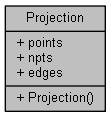
\includegraphics[width=155pt]{class_projection__coll__graph}
\end{center}
\end{figure}
\subsection*{Public Member Functions}
\begin{DoxyCompactItemize}
\item 
\mbox{\Hypertarget{class_projection_a5308ac2fb97e9805c76e3cf767f08a0e}\label{class_projection_a5308ac2fb97e9805c76e3cf767f08a0e}} 
{\bfseries Projection} (int num\+Points, float $\ast$points, bool $\ast$$\ast$edges)
\end{DoxyCompactItemize}
\subsection*{Public Attributes}
\begin{DoxyCompactItemize}
\item 
\mbox{\Hypertarget{class_projection_aa42ba5494690dbfa5f875472adc97789}\label{class_projection_aa42ba5494690dbfa5f875472adc97789}} 
float $\ast$ {\bfseries points}
\item 
\mbox{\Hypertarget{class_projection_a6972ab0bc1cfa26a5480a940d66e3497}\label{class_projection_a6972ab0bc1cfa26a5480a940d66e3497}} 
int {\bfseries npts}
\item 
\mbox{\Hypertarget{class_projection_a7943c696e88d15825dee0641b269b5f7}\label{class_projection_a7943c696e88d15825dee0641b269b5f7}} 
bool $\ast$$\ast$ {\bfseries edges}
\end{DoxyCompactItemize}


The documentation for this class was generated from the following files\+:\begin{DoxyCompactItemize}
\item 
src/model2d.\+h\item 
src/model2d.\+cpp\end{DoxyCompactItemize}

\chapter{File Documentation}
\hypertarget{_direction_cosines_8cpp}{}\section{Direction\+Cosines.\+cpp File Reference}
\label{_direction_cosines_8cpp}\index{Direction\+Cosines.\+cpp@{Direction\+Cosines.\+cpp}}
{\ttfamily \#include $<$bool$>$}\newline
{\ttfamily \#include $<$float$>$}\newline
{\ttfamily \#include $<$string$>$}\newline
{\ttfamily \#include \char`\"{}Direction\+Cosines.\+hpp\char`\"{}}\newline
{\ttfamily \#include \char`\"{}Graph.\+hpp\char`\"{}}\newline
{\ttfamily \#include \char`\"{}Line.\+hpp\char`\"{}}\newline
{\ttfamily \#include \char`\"{}Model3d.\+hpp\char`\"{}}\newline
{\ttfamily \#include \char`\"{}Orthographic\+Views.\+hpp\char`\"{}}\newline
{\ttfamily \#include \char`\"{}Plane.\+hpp\char`\"{}}\newline
{\ttfamily \#include \char`\"{}Point.\+hpp\char`\"{}}\newline
{\ttfamily \#include \char`\"{}Projection.\+hpp\char`\"{}}\newline

\hypertarget{_direction_cosines_8hpp}{}\section{Direction\+Cosines.\+hpp File Reference}
\label{_direction_cosines_8hpp}\index{Direction\+Cosines.\+hpp@{Direction\+Cosines.\+hpp}}
\subsection*{Classes}
\begin{DoxyCompactItemize}
\item 
class \mbox{\hyperlink{class_direction_cosines}{Direction\+Cosines}}
\begin{DoxyCompactList}\small\item\em Class to define the direction cosines in 3d space. \end{DoxyCompactList}\end{DoxyCompactItemize}

\hypertarget{_graph_8cpp}{}\section{Graph.\+cpp File Reference}
\label{_graph_8cpp}\index{Graph.\+cpp@{Graph.\+cpp}}
{\ttfamily \#include $<$bool$>$}\newline
{\ttfamily \#include $<$float$>$}\newline
{\ttfamily \#include $<$string$>$}\newline
{\ttfamily \#include \char`\"{}Direction\+Cosines.\+hpp\char`\"{}}\newline
{\ttfamily \#include \char`\"{}Graph.\+hpp\char`\"{}}\newline
{\ttfamily \#include \char`\"{}Line.\+hpp\char`\"{}}\newline
{\ttfamily \#include \char`\"{}Model3d.\+hpp\char`\"{}}\newline
{\ttfamily \#include \char`\"{}Orthographic\+Views.\+hpp\char`\"{}}\newline
{\ttfamily \#include \char`\"{}Plane.\+hpp\char`\"{}}\newline
{\ttfamily \#include \char`\"{}Point.\+hpp\char`\"{}}\newline
{\ttfamily \#include \char`\"{}Projection.\+hpp\char`\"{}}\newline

\hypertarget{_graph_8hpp}{}\section{Graph.\+hpp File Reference}
\label{_graph_8hpp}\index{Graph.\+hpp@{Graph.\+hpp}}
\subsection*{Classes}
\begin{DoxyCompactItemize}
\item 
class \mbox{\hyperlink{class_graph}{Graph}}
\begin{DoxyCompactList}\small\item\em A \mbox{\hyperlink{class_graph}{Graph}} Class to model a 3D or a 2D view. Determine whether to use an Adjcancey List or Adjanceny Matrix representation. \end{DoxyCompactList}\end{DoxyCompactItemize}

\hypertarget{_line_8cpp}{}\section{Line.\+cpp File Reference}
\label{_line_8cpp}\index{Line.\+cpp@{Line.\+cpp}}
{\ttfamily \#include $<$bool$>$}\newline
{\ttfamily \#include $<$float$>$}\newline
{\ttfamily \#include $<$string$>$}\newline
{\ttfamily \#include \char`\"{}Direction\+Cosines.\+hpp\char`\"{}}\newline
{\ttfamily \#include \char`\"{}Graph.\+hpp\char`\"{}}\newline
{\ttfamily \#include \char`\"{}Line.\+hpp\char`\"{}}\newline
{\ttfamily \#include \char`\"{}Model3d.\+hpp\char`\"{}}\newline
{\ttfamily \#include \char`\"{}Orthographic\+Views.\+hpp\char`\"{}}\newline
{\ttfamily \#include \char`\"{}Plane.\+hpp\char`\"{}}\newline
{\ttfamily \#include \char`\"{}Point.\+hpp\char`\"{}}\newline
{\ttfamily \#include \char`\"{}Projection.\+hpp\char`\"{}}\newline

\hypertarget{_line_8hpp}{}\section{Line.\+hpp File Reference}
\label{_line_8hpp}\index{Line.\+hpp@{Line.\+hpp}}
\subsection*{Classes}
\begin{DoxyCompactItemize}
\item 
class \mbox{\hyperlink{class_line}{Line}}
\begin{DoxyCompactList}\small\item\em A Class to define a line in the space 2\+D/3D. \end{DoxyCompactList}\end{DoxyCompactItemize}

\hypertarget{main_8cpp}{}\section{src/main.cpp File Reference}
\label{main_8cpp}\index{src/main.\+cpp@{src/main.\+cpp}}
{\ttfamily \#include \char`\"{}mainwindow.\+h\char`\"{}}\newline
{\ttfamily \#include $<$Q\+Application$>$}\newline
Include dependency graph for main.\+cpp\+:\nopagebreak
\begin{figure}[H]
\begin{center}
\leavevmode
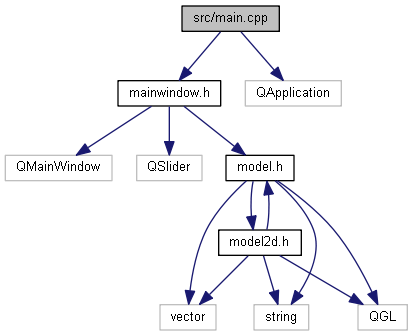
\includegraphics[width=350pt]{main_8cpp__incl}
\end{center}
\end{figure}
\subsection*{Functions}
\begin{DoxyCompactItemize}
\item 
int \mbox{\hyperlink{main_8cpp_a0ddf1224851353fc92bfbff6f499fa97}{main}} (int argc, char $\ast$argv\mbox{[}$\,$\mbox{]})
\end{DoxyCompactItemize}


\subsection{Function Documentation}
\mbox{\Hypertarget{main_8cpp_a0ddf1224851353fc92bfbff6f499fa97}\label{main_8cpp_a0ddf1224851353fc92bfbff6f499fa97}} 
\index{main.\+cpp@{main.\+cpp}!main@{main}}
\index{main@{main}!main.\+cpp@{main.\+cpp}}
\subsubsection{\texorpdfstring{main()}{main()}}
{\footnotesize\ttfamily int main (\begin{DoxyParamCaption}\item[{int}]{argc,  }\item[{char $\ast$}]{argv\mbox{[}$\,$\mbox{]} }\end{DoxyParamCaption})}


\hypertarget{_model3d_8cpp}{}\section{Model3d.\+cpp File Reference}
\label{_model3d_8cpp}\index{Model3d.\+cpp@{Model3d.\+cpp}}
{\ttfamily \#include $<$bool$>$}\newline
{\ttfamily \#include $<$float$>$}\newline
{\ttfamily \#include $<$string$>$}\newline
{\ttfamily \#include \char`\"{}Direction\+Cosines.\+hpp\char`\"{}}\newline
{\ttfamily \#include \char`\"{}Graph.\+hpp\char`\"{}}\newline
{\ttfamily \#include \char`\"{}Line.\+hpp\char`\"{}}\newline
{\ttfamily \#include \char`\"{}Model3d.\+hpp\char`\"{}}\newline
{\ttfamily \#include \char`\"{}Orthographic\+Views.\+hpp\char`\"{}}\newline
{\ttfamily \#include \char`\"{}Plane.\+hpp\char`\"{}}\newline
{\ttfamily \#include \char`\"{}Point.\+hpp\char`\"{}}\newline
{\ttfamily \#include \char`\"{}Projection.\+hpp\char`\"{}}\newline

\hypertarget{_model3d_8hpp}{}\section{Model3d.\+hpp File Reference}
\label{_model3d_8hpp}\index{Model3d.\+hpp@{Model3d.\+hpp}}
\subsection*{Classes}
\begin{DoxyCompactItemize}
\item 
class \mbox{\hyperlink{class_model3d}{Model3d}}
\begin{DoxyCompactList}\small\item\em A Representation for the 3D Model Class(isometric View) specified using a graph of nodes and edges. \end{DoxyCompactList}\end{DoxyCompactItemize}

\hypertarget{_orthographic_views_8cpp}{}\section{Orthographic\+Views.\+cpp File Reference}
\label{_orthographic_views_8cpp}\index{Orthographic\+Views.\+cpp@{Orthographic\+Views.\+cpp}}
{\ttfamily \#include $<$bool$>$}\newline
{\ttfamily \#include $<$float$>$}\newline
{\ttfamily \#include $<$string$>$}\newline
{\ttfamily \#include \char`\"{}Direction\+Cosines.\+hpp\char`\"{}}\newline
{\ttfamily \#include \char`\"{}Graph.\+hpp\char`\"{}}\newline
{\ttfamily \#include \char`\"{}Line.\+hpp\char`\"{}}\newline
{\ttfamily \#include \char`\"{}Model3d.\+hpp\char`\"{}}\newline
{\ttfamily \#include \char`\"{}Orthographic\+Views.\+hpp\char`\"{}}\newline
{\ttfamily \#include \char`\"{}Plane.\+hpp\char`\"{}}\newline
{\ttfamily \#include \char`\"{}Point.\+hpp\char`\"{}}\newline
{\ttfamily \#include \char`\"{}Projection.\+hpp\char`\"{}}\newline

\hypertarget{_orthographic_views_8hpp}{}\section{Orthographic\+Views.\+hpp File Reference}
\label{_orthographic_views_8hpp}\index{Orthographic\+Views.\+hpp@{Orthographic\+Views.\+hpp}}
\subsection*{Classes}
\begin{DoxyCompactItemize}
\item 
class \mbox{\hyperlink{class_orthographic_views}{Orthographic\+Views}}
\begin{DoxyCompactList}\small\item\em A Representation for the \mbox{\hyperlink{class_orthographic_views}{Orthographic\+Views}} Class(2\+D View) specified using a graph of nodes and edges. \end{DoxyCompactList}\end{DoxyCompactItemize}

\hypertarget{_plane_8cpp}{}\section{Plane.\+cpp File Reference}
\label{_plane_8cpp}\index{Plane.\+cpp@{Plane.\+cpp}}
{\ttfamily \#include $<$bool$>$}\newline
{\ttfamily \#include $<$float$>$}\newline
{\ttfamily \#include $<$string$>$}\newline
{\ttfamily \#include \char`\"{}Direction\+Cosines.\+hpp\char`\"{}}\newline
{\ttfamily \#include \char`\"{}Graph.\+hpp\char`\"{}}\newline
{\ttfamily \#include \char`\"{}Line.\+hpp\char`\"{}}\newline
{\ttfamily \#include \char`\"{}Model3d.\+hpp\char`\"{}}\newline
{\ttfamily \#include \char`\"{}Orthographic\+Views.\+hpp\char`\"{}}\newline
{\ttfamily \#include \char`\"{}Plane.\+hpp\char`\"{}}\newline
{\ttfamily \#include \char`\"{}Point.\+hpp\char`\"{}}\newline
{\ttfamily \#include \char`\"{}Projection.\+hpp\char`\"{}}\newline

\hypertarget{_plane_8hpp}{}\section{Plane.\+hpp File Reference}
\label{_plane_8hpp}\index{Plane.\+hpp@{Plane.\+hpp}}
\subsection*{Classes}
\begin{DoxyCompactItemize}
\item 
class \mbox{\hyperlink{class_plane}{Plane}}
\begin{DoxyCompactList}\small\item\em A Class for representation of a plane in the 3D space. \end{DoxyCompactList}\end{DoxyCompactItemize}

\hypertarget{_point_8cpp}{}\section{Point.\+cpp File Reference}
\label{_point_8cpp}\index{Point.\+cpp@{Point.\+cpp}}
{\ttfamily \#include $<$bool$>$}\newline
{\ttfamily \#include $<$float$>$}\newline
{\ttfamily \#include $<$string$>$}\newline
{\ttfamily \#include \char`\"{}Direction\+Cosines.\+hpp\char`\"{}}\newline
{\ttfamily \#include \char`\"{}Graph.\+hpp\char`\"{}}\newline
{\ttfamily \#include \char`\"{}Line.\+hpp\char`\"{}}\newline
{\ttfamily \#include \char`\"{}Model3d.\+hpp\char`\"{}}\newline
{\ttfamily \#include \char`\"{}Orthographic\+Views.\+hpp\char`\"{}}\newline
{\ttfamily \#include \char`\"{}Plane.\+hpp\char`\"{}}\newline
{\ttfamily \#include \char`\"{}Point.\+hpp\char`\"{}}\newline
{\ttfamily \#include \char`\"{}Projection.\+hpp\char`\"{}}\newline

\hypertarget{_point_8hpp}{}\section{Point.\+hpp File Reference}
\label{_point_8hpp}\index{Point.\+hpp@{Point.\+hpp}}
\subsection*{Classes}
\begin{DoxyCompactItemize}
\item 
class \mbox{\hyperlink{class_point}{Point}}
\begin{DoxyCompactList}\small\item\em A Class implementing Labelled 3D, Unlabelled 3D, Labelled 2D, Unlabelled 2D \mbox{\hyperlink{class_point}{Point}} Abstract Data Types with appropriate methods. \end{DoxyCompactList}\end{DoxyCompactItemize}

\hypertarget{_projection_8cpp}{}\section{Projection.\+cpp File Reference}
\label{_projection_8cpp}\index{Projection.\+cpp@{Projection.\+cpp}}
{\ttfamily \#include $<$bool$>$}\newline
{\ttfamily \#include $<$float$>$}\newline
{\ttfamily \#include $<$string$>$}\newline
{\ttfamily \#include \char`\"{}Direction\+Cosines.\+hpp\char`\"{}}\newline
{\ttfamily \#include \char`\"{}Graph.\+hpp\char`\"{}}\newline
{\ttfamily \#include \char`\"{}Line.\+hpp\char`\"{}}\newline
{\ttfamily \#include \char`\"{}Model3d.\+hpp\char`\"{}}\newline
{\ttfamily \#include \char`\"{}Orthographic\+Views.\+hpp\char`\"{}}\newline
{\ttfamily \#include \char`\"{}Plane.\+hpp\char`\"{}}\newline
{\ttfamily \#include \char`\"{}Point.\+hpp\char`\"{}}\newline
{\ttfamily \#include \char`\"{}Projection.\+hpp\char`\"{}}\newline

\hypertarget{_projection_8hpp}{}\section{Projection.\+hpp File Reference}
\label{_projection_8hpp}\index{Projection.\+hpp@{Projection.\+hpp}}
\subsection*{Classes}
\begin{DoxyCompactItemize}
\item 
class \mbox{\hyperlink{class_projection}{Projection}}
\begin{DoxyCompactList}\small\item\em The \mbox{\hyperlink{class_projection}{Projection}} Class which simply defines the detailed graph required for our software. \end{DoxyCompactList}\end{DoxyCompactItemize}

%--- End generated contents ---

% Index
\backmatter
\newpage
\phantomsection
\clearemptydoublepage
\addcontentsline{toc}{chapter}{Index}
\printindex

\end{document}
